\chapter{Spectroscopy of $\Sr{87}$ Triplet Rydberg States}

In order to study strontium Rydberg atoms, it's necessary to be able to locate and identify the Rydberg state being excited. 
Most spectroscopic studies of strontium Rydberg systems have focused on the most abundant isotope, \Sr{88}, which has no nuclear spin ($I = 0$). 
This lack of nuclear spin means no hyperfine structure and leads to relatively simple excitation spectra which has been well mapped and understood \cite{Esherick1977.PRA.15.1920, Beigang1982.OC.42.19, Beigang1982.PS.26.183, Kunze1993.ZPD.27.111, Dai1995.JQSRT.54.1019, Dai1995.PRA.52.4416, Philip2007.OC.279.141, Jackson2018.PhD, Couturier2019.PRA.99.022503}.

In contrast, relatively few studies have been done on \Sr{87} which has a large nuclear spin ($I = {9}/{2}$) which leads to a strong hyperfine interaction, complicating the Rydberg excitation spectrum.
Of the previous experimental work \cite{Beigang1981.ZPhys.301.93, Beigang1981.PRL.47.326, Beigang1982.PRL.48.290, Beigang1982.PRA.25.1496, Beigang1983.PRL.51.771}, excitation was performed to singlet Rydberg states ($\nSLJ{5sns}{1}{S}{0}$ and $\nSLJ{5snd}{1}{D}{2}$) with triplet states being observed due to state mixing. 
In order to better understand the \Sr{87} Rydberg spectra, we mapped the triplet Rydberg states by directly exciting $\nSLJ{5sns}{3}{S}{1}$ and $\nSLJ{5snd}{3}{D}{1,2,3}$ through the intermediate $\nSLJ{5s5p}{3}{P}{1}$ state. 
Collaborating with theorists, we were able to develop an understanding of the \Sr{87} hyperfine Rydberg states.

Below is a summary of our work, published in \cite{Ding2018.PRA.98.042505}, which was a combined experimental and theoretical study of $\nSLJ{5sns}{3}{S}{1}$ and $\nSLJ{5snd}{3}{D}{1,2,3}$ Rydberg states in \Sr{87}.
The experimental work was performed at Rice with theoretical calculations performed by Dr. Shuhei Yoshida and Dr. Joachim Burgd{\"{o}}rfer at the Institute for Theoretical Physics, Vienna University of Technology. 

\section{Ionization Limit of $\Sr{87}$}

The first indication that the Rydberg levels of $\Sr{87}$ were not as simple as for the bosonic isotopes was the reported ionization limit, $E_{\text{ion}}^{87} = \SI{45932.2861(10)}{\per\cm}$ \cite{Beigang1982.OC.42.19, Sansonetti2010.JPCRD.39.033103}, being well above those of the bosonic isotopes (see \cref{fig:Eion-mass-scaled} and \cref{tab:ionization_limits}). 
\begin{figure}[htbp]
	\centering
	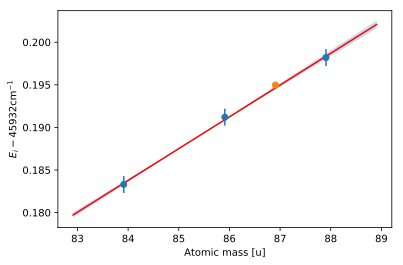
\includegraphics[keepaspectratio, width=4.5in, height=\textheight]{fermion_spectroscopy/calculations/Eion-mass-scaled.pdf}
	\caption{
		\label{fig:Eion-mass-scaled}
		(Blue points) Reported isotopic ionization limits ($E_{\text{ion}}$) vs. isotope mass.
		A linear fit (black line) is used to estimate the $E_{\text{ion}}^{87}$ for an assumed $I=0$ \Sr{87} atom from the ionization energies of the bosonic isotopes. 
		See \cref{ap:sr_data} for isotopic masses and ionization energies.}
\end{figure}
Mass-scaling the ionization energies of the bosonic isotopes suggests that the ionization energy for an assumed $I=0$ \Sr{87} atom should be $\SI{45932.1946+-0.0005}{\per\cm}$, about $\SI{2.74}{\GHz}$ below the reported ionization energy.

The source of this discrepancy is likely related to the hyperfine interaction in the ground state of \Srion{87}{+}. 
Since ground state \Srion{87}{+} has a rubidium-like structure with a single valence $s$ electron outside a filled {[Kr]} core, the hyperfine interaction can be written as (see, e.g., \cite{Steck.QuantumAtomOptics})
\begin{equation}
	\hat{V}_{\text{hfs}}	=	A_{\text{hfs}} \hat{\va{I}} \vdot \hat{\va{J}}
							=	A_{\text{hfs}} \hat{\va{I}} \vdot \hat{\va{S}}
\end{equation}
where $\va{J} = \va{L} + \va{S}$ and $A_{\text{hfs}}$ is the strength of the magnetic dipole hyperfine interaction.
Note that there are no higher order contributions (e.g., electric quadrupole) since the valence electron is in an $s$ state so only the contact interaction is non-zero \cite{Arimondo1977.RMP.49.31}.
Following the usual procedure by defining $\va{F} = \va{J} + \va{I}$, the energy shift can be evaluated as
\begin{equation}
	\ev*{\hat{V}_{\text{hfs}}}	=	\frac{A_{\text{hfs}}}{2} \ev*{\hat{\va{F}}^2 - \hat{\va{J}}^2 - \hat{\va{I}}^2}
								=	\frac{A_{\text{hfs}}}{2} \bqty{F \pqty{F + 1} - J \pqty{J + 1} - I \pqty{I + 1}}
\end{equation}
In the ground state of \Srion{87}{+}, $S=s={1}/{2}$ and $I={9}/{2}$ meaning the the $\nSLJ{5s}{2}{S}{1/2}$ is split in to $F = 4$ and $F = 5$ components.
Using $A_{\text{hfs}} = \SI{-1000473.673(11)}{\kHz}$\footnote{\citeauthor{Sunaoshi1993.HI.78.241} determined $A_{\text{hfs}}$ by measuring the splitting of the $\nSLJf{5s}{2}{S}{1/2}{4}$ and $\nSLJf{5s}{2}{S}{1/2}{5}$ ground state of \Srion{87}{+} in an ion trap. They measured the splitting to be $E_{F=4} - E_{F=5} = \SI{5002368.363(57)}{\kHz}$.} \cite{Sunaoshi1993.HI.78.241}, the $F=4$ and $F=5$ states are shifted by
\begin{equation}
	\ev*{\hat{V}_{\text{hfs}}}	=	\begin{cases}
										-\frac{11}{4} A_{\text{hfs}} = \SI{2.751302601+-0.000000030}{\GHz}	,{}&{}	F=4	\\
										\frac{9}{4} A_{\text{hfs}} = \SI{-2.251065764+-0.000000025}{\GHz}	,{}&{}	F=5
									\end{cases}
\end{equation}
Notice that $\ev*{\hat{V}_{\text{hfs}}}_{F=4}$ nearly matches the $\SI{2.74}{\GHz}$ discrepancy between the reported ionization limit of \Sr{87} and the ionization limit determined by mass-scaling from the bosonic isotopes. 
This seems reasonable since most of the earlier spectroscopic work on \Sr{87} primarily focused on the singlet Rydberg states of which converges to the upper $F = 4$ \cite{Beigang1982.PRA.25.1496} state of \Srion{87}{+}. 

In the analysis below, we used $E_{\text{ion}}^{87} = \SI{45932.1956+-0.0007}{\per\cm}$ for the ionization limit instead of the slightly lower value $E_{\text{ion}}^{87} = \SI{45932.1943+-0.0010}{\per\cm}$ obtained by subtracting $\ev*{\hat{V}_{\text{hfs}}}_{F=4}$ from the reported \Sr{87} ionization limit in \cite{Beigang1982.OC.42.19, Sansonetti2010.JPCRD.39.033103}.
As described in \cite{Ding2018.PRA.98.042505}, it was found that the higher $E_{\text{ion}}^{87}$ resulted in the quantum defects of the $\nSLJ{5sns}{1}{S}{0}$ and $\nSLJ{5sns}{3}{S}{1}$ states converging to a nearly constant value.

\section{Hyperfine Rydberg States of \Sr{87}}

Accurate \textit{ab initio} theoretical descriptions of the Rydberg structure of multielectron atoms is currently challenging due to the interaction of the Rydberg electron with the ionic core. 
This interplay may lead to different configurations (``channels'') of the Rydberg electron and the ionic core which share the same total energy, angular momentum, and parity \cite{Gallagher1994.RydbergAtoms, Vaillant2014.JPB.47.155001}.
When the ionic states are not well-separated from the Rydberg states, multichannel quantum defect theory (MQDT) is the commonly used method for analyzing the Rydberg states of these multielectron atoms which can describe the Rydberg state in terms of a few parameters \cite{Gallagher1994.RydbergAtoms, Aymar1996.RMP.68.1015, Robicheaux2018.PRA.97.022508}\footnote{I think \cite{Cooke1985.PRA.32.2725}, referenced and followed by \cite{Gallagher1994.RydbergAtoms}, would probably be a good paper to work through as they provide an example calculation.}. 

Focusing on two-electron systems (e.g., {\tsup{3}\text{He}}, {\tsup{9}\text{Be}}, {\tsup{25}\text{Mg}}, {\tsup{43}\text{Ca}}, \Sr{87}, {\tsup{135}\text{Ba}}, {\tsup{137}\text{Ba}}), we follow the approach adopted in \cite{Beigang1982.PRA.25.1496, Beigang1983.PRL.51.771, Beigang1988.JOSAB.5.2423} and separate the total Hamiltonian for the system in to a part which does not depend on the nuclear spin ($\hat{H}_{0}^{I = 0}$) and the hyperfine interaction ($\hat{V}_{\text{hfs}}$) which does depend on the nuclear spin
\begin{equation}
	\hat{H}^{I \neq 0} = \hat{H}_{0}^{I = 0} + \hat{V}_{\text{hfs}}
\end{equation}
$\ev*{\hat{H}_{0}^{I = 0}}$ contains the effects up to the fine structure level. 
The convenience of separating out the $\hat{H}_{0}^{I = 0}$ term becomes apparent because the eigenenergies (up to the fine structure level) can be obtained from the Rydberg-Ritz formula
\begin{equation}
	\label{eq:rydberg-ritz}
	\ev*{\hat{H}_{0}^{I = 0}}	=	E_{\text{ion}} - \frac{R}{\pqty{n - \mu_{n,L,S,J}}^{2}}
\end{equation}
with the quantum defect given by \cite{Gentile1990.PRA.42.440, Gallagher1994.RydbergAtoms, Vaillant2012.JPB.45.135004}\footnote{** There's an interesting discussion on how the equation for quantum defect is supposed to be recursive with $n^{*} = n - \delta\pqty{n^{*}} = n - \delta_{0} - \delta_{2}/\pqty{n - \delta}^{2} - \delta_{4}/\pqty{n - \delta}^{4} - \cdots$ \cite{Drake1991.PRA.44.5448} vs. the power-series expansion presented in \cite{Gentile1990.PRA.42.440} **.}
\begin{equation}
	\mu_{n,L,S,J}	=	\mu_{0} + \frac{\mu_{2}}{\pqty{n - \mu_{0}^{2}}^{2}} + \frac{\mu_{4}}{\pqty{n - \mu_{0}^{2}}^{4}} + \cdots
\end{equation}
Therefore, we only need to evaluate $\ev*{\hat{V}_{\text{hfs}}}$ to obtain the hyperfine shifts.

The hyperfine interaction can be expressed as \cite{Woodgate.Elementary, Sobelman.Atomic, Bransden.Atoms}
\begin{equation}
	\hat{V}_\text{hfs}	=	A \hat{\va{I}} \cdot \hat{\va{J}}
						=	\sum_{i} A_{i} \hat{\va{I}} \cdot \hat{\va{j}}_{i}
						=	\sum_{i} A_{i} \hat{\va{I}} \cdot \pqty{\hat{\va{l}}_{i} + \hat{\va{s}}_{i}}
\end{equation}
for electron $i \in \Bqty{1,2}$ with the (magnetic dipole) hyperfine constant $A$.
Therefore the contribution of each electron to the total hyperfine shift is
\begin{equation}
	\ev*{\hat{V}_\text{hfs}}_{i}	=	A_{i} \ev*{\hat{\va{I}} \cdot \hat{\va{j}}_{i}}
									=	\frac{A_{i}}{2} \bqty{f_{i} \pqty{f_{i} + 1} - I \pqty{I + 1} - j_{i} \pqty{j_{i} + 1}}
\end{equation}
We now consider a singly-excited Rydberg states where the ``inner'' electron in the $\ket{m s}$ state (i.e., an $s$ electron in the ground state of the ion) and the ``outer'' Rydberg electron in a $\ket{n \ell}$ state.
*** I don't really like this sudden transition.... ***
Recalling that the $\ev*{\hat{V}_\text{hfs}}_{i} \sim {1}/{n^{3}}$ ** \cite{Gudde1993.PRA.47.4725, Sobelman.Atomic, Bransden.Atoms} **, it follows that for high-$n$ Rydberg states, the $\ev*{\hat{V}_\text{hfs}}_{i}$ can be approximated as
\begin{align}
	\ev*{\hat{V}_\text{hfs}}_{\text{inner}}	&{}={}	A_{\text{inner}} \ev*{\hat{\va{I}} \cdot \hat{\va{s}}_{\text{inner}}}	\\
	\ev*{\hat{V}_\text{hfs}}_{\text{outer}}	&{}={}	A_{\text{outer}} \ev*{\hat{\va{I}} \cdot \hat{\va{s}}_{\text{outer}}}	\approx	0
\end{align}
Since the ``outer'' electron does not significantly contribute to $\ev*{\hat{V}_\text{hfs}}$, it follows that $\ev*{\hat{V}_\text{hfs}} \simeq \ev*{\hat{V}_\text{hfs}}_{\text{inner}}$.
Here, $A_{\text{inner}}$ is taken to be ** ? ** as the same value as $A$ in the $\nSLJ{5s}{2}{S}{1/2}$ state of \Srion{87}{+}.

Combining the above results, we can write the expected energies of the hyperfine Rydberg levels of isotopes with $I \neq 0$ as a shift from the ``unperturbed'' levels in an isotope with $I = 0$.

*** I need to come up with a better derivation.... I went down a bit of a rabbit hole above... ***

\subsection{Singly Excited $S$ states}

The calculation for the hyperfine shifts of singly excited $S$ Rydberg states is not too difficult with most of the details worked out in \cref{sec:hyperfine_mixing_derivation}. 
It can be shown that the four hyperfine basis states are $\ket{\SLJf{1}{S}{0}{I}}$, $\ket{\SLJf{3}{S}{1}{I+1}}$, $\ket{\SLJf{3}{S}{1}{I}}$, and $\ket{\SLJf{3}{S}{1}{I-1}}$.
Using these basis states, we can evaluate the matrix elements of the hyperfine interaction and find that only the $F = I$ states interact with the matrix elements \cite{Beigang1982.PRA.25.1496}
\begin{align}
	\bra{\SLJf{1}{S}{0}{I}} \hat{V}_\text{hfs} \ket{\SLJf{1}{S}{0}{I}}	&{}={}	0										\\
	\bra{\SLJf{1}{S}{0}{I}} \hat{V}_\text{hfs} \ket{\SLJf{3}{S}{1}{I}}	&{}={}	\frac{a_{ms}}{2} \sqrt{I \pqty{I+1}}	\\
	\bra{\SLJf{3}{S}{1}{I}} \hat{V}_\text{hfs} \ket{\SLJf{1}{S}{0}{I}}	&{}={}	\frac{a_{ms}}{2} \sqrt{I \pqty{I+1}}	\\
	\bra{\SLJf{3}{S}{1}{I}} \hat{V}_\text{hfs} \ket{\SLJf{3}{S}{1}{I}}	&{}={}	-\frac{a_{ms}}{2} 
\end{align}
Therefore, $\hat{H}^{I \neq 0}$ for the interacting $F = I$ states is
\begin{equation}
	\hat{H}^{I \neq 0}	=	\hat{H}^{I = 0} + \hat{V}_\text{hfs}
						=	\begin{pmatrix}
								E_{\SLJ{1}{S}{0}}	&	0					\\ 
								0					&	E_{\SLJ{3}{S}{1}}
							\end{pmatrix}
						+	\frac{a_{ms}}{2}
							\begin{pmatrix}
								0					&	\sqrt{I \pqty{I+1}}	\\ 
								\sqrt{I \pqty{I+1}}	&	-1
							\end{pmatrix}
\end{equation}
As mentioned previously, $E_{\SLJ{1}{S}{0}}$ and $E_{\SLJ{3}{S}{1}}$ can be obtained from \cref{eq:rydberg-ritz} with the appropriate quantum defects for each series. 


***************

***************

***************


For singly excited Rydberg states $\ket{\nSLJM{5snl}{2S+1}{L}{J}{m_J}}_{J}$ with the ``inner'' electron in the $\ket{5s}$ state and the Rydberg electron in the $\ket{nl}$ state, the symmetric ($+$) and antisymmetric ($-$) orbital wave functions can be written as $\ket{L,m_L}_{L\pm}=\frac{1}{\sqrt{2}}\left(\ket{ms;nl,m_L}\pm\ket{nl;ms,m_L}\right)$.
Combining the orbital and spin wave functions for singlet and triplet states are
\begin{align}
	\ket{\nSLJM{msnl}{1}{L}{J}{m_J}}_{J}	&{}={}	\frac{1}{\sqrt{2}} \left(\ket{ms;nl,m_L}+\ket{nl;ms,m_L}\right) \ket{0,0}_{S}	\notag	\\
											&{}={}	\ket{L,m_L=m_J}_{L+} \ket{0,0}_{S}	\\
	\ket{\nSLJM{msnl}{3}{L}{J}{m_J}}_{J}	&{}={}	\sum_{m_L} \sum_{m_S} \CG{L,m_L}{1,m_S}{J,m_J} \frac{1}{\sqrt{2}}\left(\ket{ms;nl,m_L}-\ket{nl;ms,m_L}\right) \ket{1,m_S}_{S}	\notag	\\
											&{}={}	\sum_{m_S} \CG{L,m_L}{1,m_S}{J,m_J} \ket{L,m_L=m_J-m_S}_{L-} \ket{1,m_S}_{S}
\end{align}
with the Clebsch–Gordan coefficients defined as $\CG{J_1,M_1}{J_2,M_2}{J,M}=\braket{J_1,M_1;J_2,M_2}{J,M}$.



***************

For singly-excited $S$ Rydberg states in strontium with the `inner'' electron in the $\ket{5 s}$ state and the ``outer'' electron in the $\ket{n \ell}$ state, the singlet and triplet basis states can be written as
\begin{align}
	\ket{\nSLJm{5sns}{1}{S}{0}{0}}	&{}={}	\frac{1}{2} \pqty{\ket{5s}\ket{ns} + \ket{}} \pqty{\ket{} - \ket{}}	\\
	\ket{\nSLJm{5sns}{3}{S}{1}{1}}	&{}={}	\\
	\ket{\nSLJm{5sns}{3}{S}{1}{0}}	&{}={}	\\
	\ket{\nSLJm{5sns}{3}{S}{1}{-1}}	&{}={}
\end{align}


***************

For singly-excited states, the hyperfine interaction of the ``outer'' electron with the core should scale as **$\sim 1/n^3$ \cite{Gudde1993.PRA.47.4725}? ** and should be negligible for high-lying states. 
We make the assumption that $\hat{V}_\text{hf} \simeq a_{ms} \hat{\bm{s}}_{\text{in}} \cdot \hat{\bm{I}}$ for singly-excited Rydberg states with inner electron $\ket{ms}$ and Rydberg electron $\ket{nl}$.
Expanding $\hat{\bm{s}}_\text{in}$ and $\hat{\bm{I}}$ in terms of ladder operators gives
\begin{equation}
	\label{eq:V_hf}
	\hat{V}_\text{hf} \simeq \frac{a_{ms}}{2} \left(\hat{s}_{\text{in},+} \hat{I}_{-} + \hat{s}_{\text{in},-} \hat{I}_{+} + 2\hat{s}_{\text{in},z} \hat{I}_{z}\right)
\end{equation}
with the usual ladder operators $\hat{J}_{\pm}=\hat{J}_{x} \pm \hat{J}_{y}$. 
Note that $\hat{V}_\text{hf}$ leaves the total spin $m_F$ unchanged, meaning it couples states of the same $m_F$. 

For a singly-excited Rydberg state where the Rydberg electron is in the $\ket{n \ell}$ state while the inner electron remains in the $\ket{m s}$ state, the Hamiltonian can be approximated as
\begin{equation}
	\hat{H} = \pqty{\hat{H}_{0} + \hat{H}_{\text{fs}} + \zeta_{nl} \hat{\va{s}} \vdot \hat{\va{l}}} + a_{ms} \hat{\va{s}} \vdot \hat{\va{I}}
\end{equation}
where $\zeta_{nl}$ is the magnitude of the spin-orbit interaction (of the Rydberg electron), and $a_{ms}$ is the strength of the hyperfine interaction of the inner $s$ electron. 
Making the assumption that the terms $\pqty{\cdots}$ are the same for all isotopes, then the remaining hyperfine shift is simply due to the contact interaction between the remaining $ms$ electron and the ion.
This allows us to leverage the simpler spectroscopic data of the bosonic isotopes from which we can deduce the eigenstates and eigenenergies of an assumed $I = 0$ atom before incorporating isotope-specific hyperfine interactions.
\begin{equation}
	\hat{H}^{I \neq 0}	=	\hat{H}_{0}^{I = 0} \pqty{m_{I = 0}, m_{I \neq 0}} + \hat{V}_{\text{hfs}}
\end{equation}
where $\hat{H}_{0}^{88} \pqty{m_{88}, m_{87}}$ is the unperturbed Hamiltonian that yields the eigenstates and eigenenergies, for \Sr{88} but scaled by the reduced mass $m_{87} = \flatfrac{m_{e} M_{87}}{\pqty{m_{e} + M_{87}}}$. $\hat{V}_{\text{hfs}}$ is the hyperfine interaction, $m_{e}$ the electron mass and $M_{87}$ the mass of the \Srion{87}{+} ion.

Focusing on strontium, corrections beyond the elementary isotope shift, in particular, the mass polarization correction, was estimated from earlier data for helium Rydberg states \cite{Cok1979.PRA.19.1830, Cok1981.PRA.24.3283, vanderVeldt1990.PRA.41.4099} and are expected to be $\lesssim \SI{1}{\MHz}$ and are neglected.
Under this assumption, the energies of the \Sr{87} Rydberg states should be given by
\begin{equation}
	\ev*{\hat{H}^{87}}	=	\ev*{\hat{H}_{0}^{88} \pqty{m_{88}, m_{87}}} + \ev*{\hat{V}_{\text{hfs}}}
\end{equation}
The values of $\ev*{\hat{H}_{0}^{88} \pqty{m_{88}, m_{87}}}$ are easily determined from the Rydberg-Ritz formula
\begin{equation}
	\label{eq:rydberg-ritz}
	\ev*{\hat{H}^{87}}	=	\ev*{\hat{H}_{0}^{88} \pqty{m_{88}, m_{87}}}
						=	E^{87}_{\text{ion}} - \frac{R^{87}_{\text{Sr}}}{\pqty{n - \mu_{n,L,S,J}}^{2}}
\end{equation}
with the quantum defect given by ** \cite{Gentile1990.PRA.42.440, Gallagher1994.RydbergAtoms, Vaillant2012.JPB.45.135004} cite just Gallagher and Vaillant paper? **
\begin{equation}
	\mu_{n,L,S,J}	=	\mu_{0} + \frac{\mu_{2}}{\pqty{n - \mu_{0}^{2}}^{2}} + \frac{\mu_{4}}{\pqty{n - \mu_{0}^{2}}^{4}}
\end{equation}
** Use footnote? There's an interesting discussion on how the equation for quantum defect is supposed to be recursive with $n^{*} = n - \delta\pqty{n^{*}} = n - \delta_{0} - \delta_{2}/\pqty{n - \delta}^{2} - \delta_{4}/\pqty{n - \delta}^{4} - \cdots$ \cite{Drake1991.PRA.44.5448} vs. the power-series expansion presented in \cite{Gentile1990.PRA.42.440}. **

An important consideration in determining when effects cannot be neglected is when the energy scales become comparable.
For tstrontium, the energy scale of the hyperfine interaction is given by $a_{5s}$ and, as $n$ increases this energy scale becomes comparable.
As seen in \cref{fig:n-scaling}, it first becomes comparable to the fine structure splitting, then the singlet-triplet splitting, then the Coulomb splitting.
\begin{figure}[htbp]
	\centering
	\includesvg[keepaspectratio, width=\textwidth, height=\textheight]{fermion_spectroscopy/calculations/n-scaling.svg}
	\caption{
		\label{fig:n-scaling}
		The $n$ scaling of various splittings in \Sr{88} calculated using the most recently reported quantum defects and ionization energy \cite{Vaillant2012.JPB.45.135004, Couturier2019.PRA.99.022503}.
		The energy scale of the hyperfine interaction in \Sr{87} is approximately constant and is $\abs{a_{5s}} \approx \SI{1}{\GHz}$ \cite{Sunaoshi1993.HI.78.241}.
		The splittings between various states are represented by $\Delta E^{\pqty{0}}_{X}$ between the given states where $X=S$ is the singlet-triplet splitting, $X=J$ is the fine structure splitting, and $X=n$ is the Coulomb splitting.}
\end{figure}
From \cref{fig:n-scaling}, one would also expect hyperfine mixing to occur between $n \sim 10$ and $n \sim 20$ which was indeed observed \cite{Beigang1981.PRL.47.326, Beigang1982.PRL.48.290, Vaillant2014.JPB.47.155001}.
Hyperfine mixing was also observed between the $\nSLJ{5s19d}{1}{D}{2}$ and $\nSLJ{5s19d}{3}{D}{3}$ states \cite{Beigang1982.JPB.15.L201}.

%\subsection{Singly Excited $S$ states}

In the below, we follow the derivation outlined in \cite{Beigang1982.PRA.25.1496,Beigang1983.PRL.51.771}.
A more detailed derivation is provided in \cref{sec:hyperfine_mixing_derivation} where it is shown that $\hat{V}_\text{hf}$ only mixes states of the same $F$.
** I need to actually do the derivation.... **

Assuming there are no perturbing states, a reasonable assumption for $n \gtrsim 12$ for the both the $\nSLJ{5sns}{1}{S}{0}$ and $\nSLJ{5sns}{3}{S}{1}$ Rydberg series \cite{Vaillant2014.JPB.47.155001}, we start with the pure singly-excited singlet $\ket{\SLJf{1}{S}{0}{I}}$ and triplet $\ket{\SLJf{3}{S}{1}{I+1}}$, $\ket{\SLJf{3}{S}{1}{I}}$, and $\ket{\SLJf{3}{S}{1}{I-1}}$ hyperfine states.
Applying $\hat{V}_\text{hf}$ to these basis states gives
\begin{align}
	&	\hat{V}_\text{hf} \ket{\SLJf{3}{S}{1}{I+1}}	=	\frac{1}{2} a_{5s} I \ket{\SLJf{3}{S}{1}{I+1}}	\\
	&	\hat{V}_\text{hf} \ket{\SLJf{1}{S}{0}{I}}	=	\frac{1}{2} a_{5s} \sqrt{I\qty(I+1)} \ket{\SLJf{3}{S}{1}{I}}	\\
	&	\hat{V}_\text{hf} \ket{\SLJf{3}{S}{1}{I}}	=	\frac{1}{2} a_{5s} \qty(\sqrt{I\qty(I+1)} \ket{\SLJf{1}{S}{0}{I}} - \ket{\SLJf{3}{S}{1}{I}})	\\
	&	\hat{V}_\text{hf} \ket{\SLJf{3}{S}{1}{I-1}}	=	-\frac{1}{2} a_{5s} \qty(I+1) \ket{\SLJf{3}{S}{1}{I-1}}
\end{align}
From the above, it's apparent that the unmixed states have energy shifts
\begin{equation}
	\bra{\SLJf{3}{S}{1}{I+1}} \hat{V}_\text{hf} \ket{\SLJf{3}{S}{1}{I+1}}	=	\frac{1}{2} a_{5s} I			\approx	\SI{-2.25}{\GHz}
\end{equation}
\begin{equation}
	\bra{\SLJf{3}{S}{1}{I-1}} \hat{V}_\text{hf} \ket{\SLJf{3}{S}{1}{I-1}}	=	-\frac{1}{2} a_{5s} \qty(I+1)	\approx	\SI{2.75}{\GHz}
\end{equation}
The matrix elements of the mixed $F=I$ states are
\begin{equation}
	\bra{\SLJf{1}{S}{0}{I}} \hat{V}_\text{hf} \ket{\SLJf{1}{S}{0}{I}}	=	0
\end{equation}
\begin{equation}
	\bra{\SLJf{3}{S}{1}{I}} \hat{V}_\text{hf} \ket{\SLJf{3}{S}{1}{I}}	=	-\frac{1}{2} a_{5s}
\end{equation}
\begin{equation}
	\bra{\SLJf{3}{S}{1}{I}} \hat{V}_\text{hf} \ket{\SLJf{1}{S}{0}{I}}	=	\frac{1}{2} a_{5s} \sqrt{I\qty(I+1)}
\end{equation}
Therefore $F=I$ submatrix of the block-diagonal $\hat{V}_\text{hf}$ matrix can be written as
\begin{equation}
	\hat{V}_\text{hf}	=	\frac{1}{2} a_{5s}
							\begin{pmatrix}
								0							& \sqrt{I\left(I+1\right)}	\\ 
								\sqrt{I\left(I+1\right)}	& -1						\\ 
							\end{pmatrix}
\end{equation}
Diagonalizing the total Hamiltonian $\hat{H} = \hat{H}_0 + \hat{V}_\text{hf}$ gives the eigenenergies
\begin{equation}
	E^{\pm}	=	\frac{E_{1}+E_{3}}{2} - \frac{1}{4} a_{5s} \pm \frac{1}{2} \sqrt{\qty(E_{1}-E_{3})^2 + a_{5s} \qty(E_{1}-E_{3}) + a_{5s}^{2} \qty(I + \frac{1}{2})^2}
\end{equation}
Taking the limit $a_{5s} \rightarrow 0$ (i.e., no hyperfine interaction), we observe $E^{+} \rightarrow E\qty(\SLJ{1}{S}{0})$ and $E^{-} \rightarrow E\qty(\SLJ{3}{S}{1})$ meaning $E^{+}$ corresponds to the energy of $\ket{\nSLJf{5sns}{1}{S}{0}{9/2}}$ and $E^{+}$ corresponds to energy of $\ket{\nSLJf{5sns}{3}{S}{1}{9/2}}$.

\subsubsection{$n$-mixing}

At higher $n$, the hyperfine shift becomes comparable to the splitting between $n$ and $n^{\prime} = n \pm 1$ as seen in \cref{fig:n-scaling}. 
Hyperfine-induced $n$-mixing was experimentally observed around $n = \num{113}$ between the $\nSLJf{5sns}{1}{S}{0}{9/2}$ and $\nSLJf{5s\qty(n+1)s}{3}{S}{1}{9/2}$ states \cite{Beigang1983.PRL.51.771}.

The derivation above can be extended to incorporate $n$-mixing. 
Using the fact that $\hat{V}_\text{hf}$ only couples states with the same $F$ and the orthogonality of the radial wave functions for states of same spin multiplet but different $n$, the diagonal matrix elements of $\hat{V}_\text{hf}$ for $\nSLJf{5sns}{3}{S}{1}{I+1}$ and $\nSLJf{5sns}{3}{S}{1}{I-1}$ can be written as
\begin{equation}
	\mel{\nSLJf{5sn^{\prime}s}{3}{S}{1}{I+1}}{\hat{V}_\text{hf}}{\nSLJf{5sns}{3}{S}{1}{I+1}}	=	\frac{1}{2} a_{5s} I \delta_{n,n^{\prime}}
\end{equation}
\begin{equation}
	\mel{\nSLJf{5sn^{\prime}s}{3}{S}{1}{I-1}}{\hat{V}_\text{hf}}{\nSLJf{5sns}{3}{S}{1}{I-1}}	=	-\frac{1}{2} a_{5s} \qty(I+1) \delta_{n,n^{\prime}}
\end{equation}
The off-diagonal elements vanish between these states because they remain uncoupled.


****** I don't think I can do this ``expansion''... I think I want to just calculate matrix elements between n and n' states ******
On the other hand, because $\hat{V}_\text{hf}$ mixes the $\nSLJf{5sns}{1}{S}{0}{I}$ and $\nSLJf{5sns}{3}{S}{1}{I}$ states, we can write
\begin{align}
	\ket{\nSLJf{5sns}{1}{S}{0}{I}}	{}={}&	\ket{\nSLJf{n}{1}{S}{0}{I}} + \sum_{n^{\prime}}{\ket{\nSLJf{n^{\prime}}{3}{S}{1}{I}}}	\\
	\ket{\nSLJf{5sns}{3}{S}{1}{I}}	{}={}&	\ket{\nSLJf{n}{3}{S}{1}{I}} + \sum_{n^{\prime}}{\ket{\nSLJf{n^{\prime}}{1}{S}{0}{I}}}
\end{align}
where $\nSLJf{n}{1}{S}{0}{I}$ and $\nSLJf{n}{3}{S}{1}{I}$ represent pure singly-excited singlet and triplet $F=I$ states (recalling that the radial wave functions are orthogonal for $n \neq n^{\prime}$ for states in the same spin multiplet).
Calculating the matrix elements of $\hat{V}_\text{hf}$ between $\nSLJf{5sns}{1}{S}{0}{I}$ and $\nSLJf{5sns}{3}{S}{1}{I}$ gives
\begin{equation}
	\mel{\nSLJf{5s{n^\prime}s}{1}{S}{0}{I}}{\hat{V}_\text{hf}}{\nSLJf{5sns}{1}{S}{0}{I}}	=	0
\end{equation}
\begin{equation}
	\mel{\nSLJf{5s{n^\prime}s}{3}{S}{1}{I}}{\hat{V}_\text{hf}}{\nSLJf{5sns}{3}{S}{1}{I}}	=	-\frac{1}{2} a_{5s} \delta_{n,n^{\prime}}
\end{equation}
The off-diagonal elements can be expressed as
\begin{align}
	\mel{\nSLJf{5s{n^\prime}s}{1}{S}{0}{I}}{\hat{V}_\text{hf}}{\nSLJf{5sns}{3}{S}{1}{I}}
		{}={}&	-\frac{1}{2} a_{5s} (stuff to finish deriving)	\notag	\\
		{}={}&	-\frac{1}{2} a_{5s} \sqrt{I \qty(I+1)} O_{n,n^{\prime}}
\end{align}
where $O_{n,n^{\prime}}$ is the overlap between the singlet and triplet radial wave functions which can be estimated semiclassically \cite{Bhatti1981.PRA.24.161, Beigang1983.PRL.51.771}
\begin{equation}
	O_{n_{1},n_{2}}
		=	\braket{n_{1}^{*}}{n_{2}^{*}}
		=	\qty(-1)^{n_{2}-n_{1}} \frac{2 \sqrt{n_{1}^{*} n_{2}^{*}}}{n_{1}^{*} + n_{2}^{*}} \frac{\sin[\pi \qty(n_{2}^{*} - n_{1}^{*})]}{\pi \qty(n_{2}^{*} - n_{1}^{*})}
\end{equation}

\begin{figure}[htbp]
	\centering
	\includesvg[keepaspectratio, width=5in, height=\textheight]{fermion_spectroscopy/calculations/s-states/semiclassical_overlap.svg}
	\caption{
		\label{fig:semiclassical_overlap}
		** FIX FIGURE Y-AXIS LABELS **.
		Semiclassical estimation of the radial wave function overlap \cite{Bhatti1981.PRA.24.161} between $\nSLJ{n}{1}{S}{0}$ and $\nSLJ{n^{\prime}}{3}{S}{1}$ states ($O_{n,n^{\prime}}$) for $n^{\prime}=n, n+1, n+2$.}
\end{figure}

Between adjacent $n$ (i.e., for $n_{2} = n_{1} + 1$) and $\delta_{2} \neq \delta_{1}$, the approximation reduces to
\begin{equation}
	O_{n_{1},n_{1}+1}
		=	\braket{n_{1}^{*}}{\qty(n_{1}+1)^{*}}
		=	-\frac{2 \sqrt{n_{1}^{*} \qty(n_{1}+1)^{*}}}{n_{1}^{*} + \qty(n_{1}+1)^{*}} \frac{\sin[\pi \qty(\qty(n_{1}+1)^{*} - n_{1}^{*})]}{\pi \qty(\qty(n_{1}+1)^{*} - n_{1}^{*})}
\end{equation}
Since the $\nSLJf{5sns}{1}{S}{0}{9/2}$ state is always higher in energy than the $\nSLJf{5sns}{3}{S}{1}{9/2}$, they should cross when $n_{1}$ corresponds to the singlet state and $n_{2} = n_{1} + 1$ corresponds to the triplet state. 
Using the quantum defects from \cite{Vaillant2012.JPB.45.135004}, we expect $\braket{n_{1}^{*}}{\qty(n_{1}+1)^{*}} \approx \num{0.1}$ and $\braket{n_{1}^{*}}{\qty(n_{1}+1)^{*}} \approx \num{0.05}$ so we only include $n$ and $n+1$ mixing.

As see in \cref{fig:semiclassical_overlap}, the strongest $n$-mixing occurs for $\Delta n = \pm 1$ with $O_{n,n^{\prime}} \approx \num{0.1}$ and quickly drops off for larger $\Delta n$. 

************************
\begin{align}
	\mel{\nSLJ{n}{1}{S}{0}}{\hat{V}_\text{hf}}{\nSLJ{n+1}{3}{S}{1}}
		&{}={}	\qty(\bra{n^{*}_{\SLJ{1}{S}{0}}}\bra{\SLJ{1}{S}{0}}) \hat{V}_\text{hf} \qty(\ket{\SLJ{3}{S}{1}}\ket{\qty(n+1)^{*}_{\SLJ{3}{S}{1}}})	\\
		&{}={}	\braket{n^{*}_{\SLJ{1}{S}{0}}}{\qty(n+1)^{*}_{\SLJ{3}{S}{1}}} \bra{\SLJ{1}{S}{0}}\hat{V}_\text{hf}\ket{\SLJ{3}{S}{1}}
\end{align}

\begin{align}
	\mel{\nSLJ{n}{1}{S}{0}}{\hat{V}_\text{hf}}{\nSLJ{n+1}{3}{S}{1}}
		{}={}	&	\bra{\nSLJ{n}{1}{S}{0}} \qty[\hat{V}_\text{hf} \ket{\nSLJ{n+1}{3}{S}{1}}]	\\
		{}\neq{}&	\frac{1}{2} a_{5s} \bra{\nSLJ{n}{1}{S}{0}} \qty[\sqrt{I \qty(I+1)} \ket{\nSLJ{n+1}{1}{S}{0}} - \ket{\nSLJ{n+1}{3}{S}{1}}]	\\
		{}={}	&	\frac{1}{2} a_{5s} \sqrt{I \qty(I+1)} \braket{\nSLJ{n}{1}{S}{0}}{\nSLJ{n+1}{1}{S}{0}}	\notag	\\
				&	- \frac{1}{2} a_{5s} \braket{\nSLJ{n}{1}{S}{0}}{\nSLJ{n+1}{3}{S}{1}}	\\
		{}={}	&	\frac{1}{2} a_{5s} \sqrt{I \qty(I+1)} \braket{n^{*}_{\SLJ{1}{S}{0}}}{\qty(n+1)^{*}_{\SLJ{1}{S}{0}}} \braket{\SLJ{1}{S}{0}}{\SLJ{1}{S}{0}}		\notag	\\
				&	- \frac{1}{2} a_{5s} \braket{n^{*}_{\SLJ{1}{S}{0}}}{\qty(n+1)^{*}_{\SLJ{3}{S}{1}}} \braket{\SLJ{1}{S}{0}}{\SLJ{3}{S}{1}}	\\
		{}={}	&	0
\end{align}

\begin{equation}
	\bra{\nSLJ{n}{1}{S}{0}} \hat{V}_\text{hf} \qty(\sum_{n^\prime}\ket{\nSLJ{n^\prime}{3}{S}{1}})	=	...
\end{equation}

************************

\subsection{Singly Excited $D$ states}

Even before including hyperfine interactions, the spin-orbit interactions leads to a breakdown of $LS$ coupling and mixes the $\SLJ{1}{D}{2}$ and $\SLJ{3}{D}{2}$ states and is especially strong around $n = \num{15}$ where they swap singlet and triplet character \cite{Esherick1977.PRA.15.1920, Beigang1981.PRL.47.326, Beigang1982.PRL.48.290, Gudde1993.PRA.47.4725, Vaillant2014.JPB.47.155001}.
To account for this mixing, the eigenstates $\nSLJ{5sns}{1}{D}{2}$ and $\nSLJ{5sns}{3}{D}{2}$ of the $H_{0}\qty(88, m_{87})$ are expanded as
\begin{align}
	\ket{\nSLJ{5sns}{1}{D}{2}}	&{}={}	\cos\theta\ket{\nSLJ{n}{1}{D}{2}} + \sin\theta\ket{\nSLJ{n}{3}{D}{2}} \\
	\ket{\nSLJ{5sns}{3}{D}{2}}	&{}={}	-\sin\theta\ket{\nSLJ{n}{1}{D}{2}} + \cos\theta\ket{\nSLJ{n}{3}{D}{2}}
\end{align}
where $\theta$ is the mixing angle \cite{Sun1989.JPB.22.2887} of the pure singlet $\ket{\nSLJ{n}{1}{D}{2}}$ and triplet $\ket{\nSLJ{n}{3}{D}{2}}$ states.
*** For higher $n$, the singlet-triplet mixing of the $\SLJ{1}{D}{2}$ and $\SLJ{3}{D}{2}$ states becomes nearly $n$ independent as evidenced by their quantum defects \cite{Vaillant2012.JPB.45.135004, Couturier2019.PRA.99.022503}. **
Calculations using a two-active-electron (TAE) model \cite{Ye2013.PRA.88.043430, Fields2018.PRA.97.013429} estimates that converges towards $\theta \sim \num{-0.16}$ for high $n$.
** Where does $\theta \sim \num{-0.14}$ come from? **

** See \cite{Gudde1993.PRA.47.4725} for a calculation of mixing coefficients? **

Calculating the hyperfine matrix elements of the $D$ states is quite a bit more challenging than for the $S$ states. 
In total, there are $\num{20}$ singly excited $D$ states ($\nSLJ{5snd}{1}{D}{2}$, $\nSLJ{5snd}{3}{D}{1}$, $\nSLJ{5snd}{3}{D}{2}$, and $\nSLJ{5snd}{3}{D}{3}$) which each have $2 I + 1 = 10$ nuclear spin states. 
The matrix elements of $\hat{V}_{\text{hfs}}$ can be evaluated analytically \cite{Lurio1962.PR.126.1758, Sun1989.JPB.22.2887, Gudde1993.PRA.47.4725}.

Due to these interactions, it's not clear how to assign the different states since $S$ and $J$ are no longer good quantum numbers. 
Instead, the state assignments were made by evaluating the overlap of the hyperfine-mixed states with the unperturbed $\nSLJ{5sns}{2S+1}{D}{J}$ state.
** CLARIFY I need to check with Shuhei that I'm understanding this correctly **


\section{Experimental Method}

A schematic diagram of the present experimental arrangement is presented in \cref{fig:spectroscopy_exp_setup}.
\begin{figure}[htbp]
	\centering
	\includesvg[keepaspectratio, width=\textwidth, height=\textheight]{fermion_spectroscopy/experiment/exp_setup.svg}
	\caption{
		\label{fig:spectroscopy_exp_setup}
		{(a)} Diagram of the experimental arrangement showing the $\SI{461}{\nm}$ cooling beams and the counterpropagating $\SI{689}{\nm}$ and $\SI{319}{\nm}$ Rydberg excitation lasers.
		{(b)} Two-photon excitation schemes utilizing either the {(\romannumeral 1)~${\nSLJf{5s5p}{3}{P}{1}{11/2}}$} or {(\romannumeral 2)~$\nSLJf{5s5p}{3}{P}{1}{9/2}$} intermediate states. 
		The detunings relative to these intermediate states are fixed at $\Delta_{11/2} \approx \SI{12}{\MHz}$ and $\Delta_{9/2} \approx \SI{36}{\MHz}$.
		{(c)} Arrangement of the electrodes used for ionizing Rydberg atoms and guiding the electrons towards the MCP detector.}
\end{figure}
The cooling and trapping of strontium was described previously in this thesis so it will only be briefly covered here. 
Following the standard procedure for laser cooling strontium, we start from a Zeeman slowed atomic beam with the Zeeman laser tuned to $\SLJ{1}{S}{0} \rightarrow \SLJ{1}{P}{1}$ resonance in \Sr{87}.
The slowed atoms are then captured by a blue MOT operating on the same transition which traps and cools the atoms to $\sim \SI{2}{\milli\kelvin}$. 
Further cooling is achieved in a narrow-line red MOT driving the $\SLJ{1}{S}{0} \rightarrow \SLJ{3}{P}{1}$ transition.
Approximately $\SI{1E6}{atoms}$ at $\sim \SI{2}{\micro\kelvin}$ are captured and cooled before turning off all trapping fields for spectroscopy measurements.

Rydberg atoms are created by two-photon excitation using counterpropagating cross-linearly polarized $\SI{689}{\nm}$ and $\SI{319}{\nm}$ excitation lasers which drive transitions to the $\nSLJ{5sns}{3}{S}{1}$ and $\nSLJ{5snd}{3}{D}{1,2,3}$ Rydberg levels via the intermediate $\nSLJf{5s5p}{3}{P}{1}{9/2}$ or $F = 11/2$ states.
These intermediate states were selected to take advantage of selection rules to aid in identifying the Rydberg hyperfine states populated.
The typical detunings of the $\SI{689}{\nm}$ laser were fixed at $\Delta_{9/2} \approx \SI{36}{MHz}$ and $\Delta_{11/2} \approx \SI{12}{\MHz}$ relative to the intermediate states.
During excitation, the $\SI{319}{\nm}$ laser was kept on while the $\SI{689}{\nm}$ laser was chopped into $\SIrange[range-phrase=-]{10}{20}{\us}$-long pulses to generate temporally localized groups of Rydberg atoms. 
The number of Rydberg atoms produced by each pulse was determined by using the electrodes in \cref{fig:spectroscopy_exp_setup} to generate a ramped electric field sufficient to ionize the Rydberg atoms with the resulting electrons directed towards, and detected by, a micro-channel plate (MCP) whose output was fed into a multichannel scalar (MCS).
Typically $\numrange[range-phrase=-]{100}{500}$ measurement cycles were performed before loading a new sample and changing the $\SI{319}{\nm}$ laser frequency. 
Spectroscopic measurements at high~$n$ using \Sr{84} showed that the stray fields in the trapping region were less than $\SI{10}{\mV\per\cm}$ so any resultant Stark shifts should be at most a few megahertz even at $n \sim 90$.

The $\SI{319}{\nm}$ radiation was generated by frequency doubling the output of a $\SI{638}{\nm}$ optical parametric oscillator (OPO). 
A sample of the output is sent though a broadband fiber electro-optic modulator (fEOM) from which one of the tunable sidebands was locked to a transfer cavity, allowing the $\SI{319}{\nm}$ laser to be scanned over multiple gigahertz.
The transfer cavity was stabilized using a $\SI{689}{\nm}$ laser locked to the $\nSLJ{5s^2}{1}{S}{0} \rightarrow \nSLJ{5s5p}{3}{P}{1}$ transition in \Sr{88}. 
The linewidth of the $\SI{319}{\nm}$ laser is estimated to be $\lesssim \SI{500}{\kHz}$ based on the narrowest observed spectroscopic features.
The Rydberg state energies are determined by measuring the $\SI{638}{\nm}$ frequency with an EXFO WA-1500 wavemeter and is resolution-limited to about $\approx \SI{60}{\MHz}$. 
Relative measurements of line splittings can be obtained to kilohertz-level accuracies when scanning within a single free spectral range (FSR) of the transfer cavity and to megahertz-level accuracies when piecing together scans over successive FSR\footnote{We have since developed a method which can provide kilohertz-level accuracies over successive FSRs without needing an accurate measurement of the FSR.}.
% Other version using lesssim in \SI: $\SI[input-comparators=\lesssim]{\lesssim500}{\kHz}$

\subsection{Calibrating the EXFO WA-1500 Wavemeter}

All light used in the calibration measurements were delivered to the EXFO WA-1500 using single mode fiber\footnote{Thorlabs SM600 FC/PC single mode fiber.}.
We had previously used a multimode fiber but found that the wavemeter readings were inconsistent, likely due to the speckle pattern or slight beam pointing deviations from output of the multimode fiber.
Switching to a single mode fiber alleviated these issue and we were able to consistently obtain resolution-limited measurements of the wavenumber with a statistical uncertainty of about $\sigma_{\text{stat}} = \pm \SI{15}{MHz}$ for the wavelengths we measured. Since the $\SI{319}{\nm}$ light is generated by frequency-doubling from $\SI{638}{\nm}$, the statistical uncertainty is approximately doubled as well $\sigma_{\text{stat}} = \pm \SI{30}{MHz}$.

Since we rely on the wavemeter to determine the absolute energy of the $\SI{638}{\nm}$ photon, we also needed to characterize potential systematics.
We initially attempted to perform Doppler-free spectroscopy of molecular iodine ({\tsup{127}I\tsub{2}}) using the ${P65~\left(7–4\right)}$ line at \SI{15672.517398(25)}{\per\cm} \cite{Sansonetti1997.JOSAB.14.1913} which is near the wavelength required to excite the $\nSLJ{5s40s}{3}{S}{1}$ Rydberg state.
We didn't have much luck observing narrow Doppler-free signals scanning the $\SI{638}{\nm}$ laser through a our iodine cell using a simple saturated absorption setup\footnote{This matches similar experiences according to Jason Nguyen and Henry Luo in the Hulet lab when they were looking to use an iodine cell to lock their $\SI{646}{\nm}$ laser for a \Li{6} UV MOT \cite{Duarte2011.PRA.84.061406}.}.
A longer cell and a more sensitive detection method may be necessary since most {\tsup{127}I\tsub{2}} spectroscopy setups in this wavelength range used cells longer than $\SI{30}{\cm}$ and some sort of modulation spectroscopy (e.g., \cite{Sansonetti1997.JOSAB.14.1913, Huang2018.AO.57.2102, Onishchenko2019.PRA.99.052503}).

Although the iodine spectroscopy didn't work out, we were able to calibrate the wavemeter by measuring wavelengths of lasers lock to atomic transitions in \Sr{88} ($\SI{689}{\nm}$) and \Li{6} ($\SI{671}{\nm}$ and $\SI{646}{\nm}$).
The $\SI{689}{\nm}$ reference comes from our red master laser locked to the $\SLJ{1}{S}{0} \rightarrow \SLJ{3}{P}{1}$ in \Sr{88}.
Ya-Ting Chang, Danyel Cavazos, and Dr. Randy Hulet were kind enough to let us run a fiber between the Killian and Hulet labs in order to measure the wavelengths of their $\SI{671}{\nm}$ and $\SI{646}{\nm}$ lasers for laser cooling \Li{6}. 
The $\SI{671}{\nm}$ is used for a standard $D_{2}$ MOT while the $\SI{646}{\nm}$ is frequency doubled to $\SI{323}{\nm}$ for a UV MOT \cite{Duarte2011.PRA.84.061406}.
The wavemeter measurements of those three wavelengths were performed within about $\SI{2}{\hour}$ to reduce sensitivity to environmental changes and are presented in \cref{tab:wavemeter_calibration}.
\begin{table}[htbp]
	\caption{
		\label{tab:wavemeter_calibration}
		Values used to calibrate the WA-1500 on a single day (2018/03/09) within about \SI{2}{\hour}. 
		The value of the \SI{689}{\nm} transition in \Sr{88} \cite{Ferrari2003.PRL.91.243002, Sansonetti2010.JPCRD.39.033103}.
		The values of the \SI{671}{\nm} and \SI{323}{\nm} (\SI{646}{\nm}) transitions in \Li{6} were taken from \cite{Sansonetti2011.PRL.107.023001, Sansonetti2012.PRL.109.259901, Radziemski1995.PRA.52.4462}.}
	\centering
	\makebox[\textwidth][c]{
	\begin{tabular}{@{}ccccc@{}}
		\toprule
		$\lambda$ [\si{\nm}]	& Atom						& Transition																		& Reference [\si{\per\cm}]			& Measured [\si{\per\cm}]		\\
		\midrule
		\num{689}				& \Sr{88}					& $\nSLJ{5s^2}{1}{S}{0} \rightarrow \nSLJ{5s5p}{3}{P}{1}$							& \num{14504.33824159+-0.00000033}	& \num{14504.34224+-0.00035}	\\
		\num{671}				& \Li{6}					& $\nSLJf{2s}{2}{S}{1/2}{3/2} \rightarrow \nSLJ{2p}{2}{P}{3/2}$						& \num{14903.6295242+-0.0000007}	& \num{14903.63391+-0.00033}	\\
		\num{323}				& \multirow{2}{*}{\Li{6}}	& \multirow{2}{*}{$\nSLJf{2s}{2}{S}{1/2}{3/2} \rightarrow \nSLJ{3p}{2}{P}{3/2}$}	& \num{30925.1703+-0.0010}			& \num{30925.1792+-0.0010}		\\
		(\num{646})				&							&																					& (\num{15462.5851+-0.0005})		& (\num{15462.5896+-0.0005})	\\
		\bottomrule
	\end{tabular}
	}
\end{table}
These measurements were used to calculate the frequency offset $\delta\pqty{\lambda} = \nu_{\text{measured}} - \nu_{\text{reference}}$ between the measured and reported values and is plotted in \cref{fig:wm_fit}.
\begin{figure}[htbp]
	\centering
	%\includesvg[keepaspectratio, width=\textwidth]{fermion_spectroscopy/wavemeter_calibration/wm_fit.svg}
	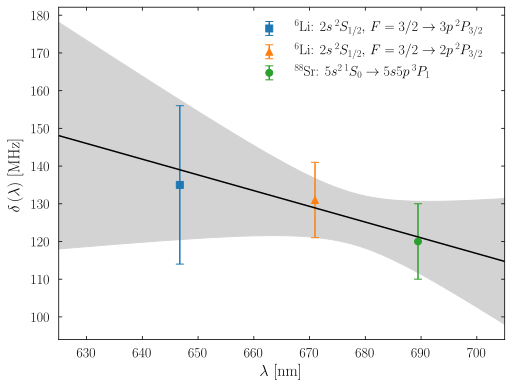
\includegraphics[keepaspectratio, width=4.5in]{fermion_spectroscopy/wavemeter_calibration/wm_fit.pdf}
	\caption{
		\label{fig:wm_fit}
		Wavelength dependence of the offset between the measured and published transition frequencies used to calibrate the wavemeter $\delta\pqty{\lambda} = \nu_{\text{measured}} - \nu_{\text{reference}}$. 
		The black line shows the linear fit used to obtain the offset at $\SI{638}{\nm}$ with the shaded region representing the uncertainty in the wavemeter calibration obtained from Monte Carlo simulations.}
\end{figure}
A linear fit yields a correction of $\approx \SI{140}{\MHz}$ at $\SI{638}{\nm}$. 
In an attempt to estimate the systematic uncertainty in this calibration factor, a Monte Carlo sampling was adopted in which linear fits to points drawn at random from a Gaussian distributions appropriate to each point in the calibration were repeated, resulting in a systematic uncertainty of about $\sigma_{\text{sys}} = \pm \SI{25}{\MHz}$ ($\sigma_{\text{sys}} = \pm \SI{50}{\MHz}$) at $\SI{638}{\nm}$ ($\SI{319}{\nm}$). 

To check for drifts in the wavemeter calibration, each $\SI{638}{\nm}$ wavelength measurement was followed by a reference measurement of the $\SI{689}{\nm}$ master laser.
As shown in \cref{fig:wm_drift}, the day-to-day variations were relatively small compared to the wavemeter's systematic uncertainty which we suspect are due to changes in environmental conditions (e.g., temperature, humidity, pressure).
\begin{figure}[htbp]
	\centering
	%\includesvg[keepaspectratio, width=\textwidth]{fermion_spectroscopy/wavemeter_calibration/wm_drift.svg}
	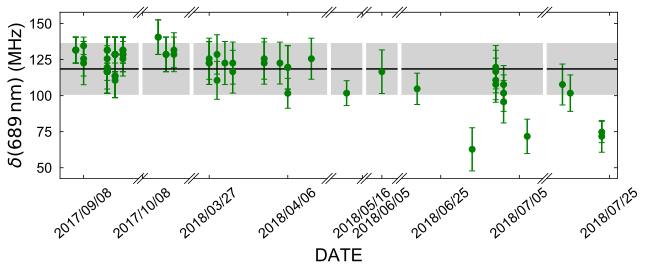
\includegraphics[keepaspectratio, width=\textwidth]{fermion_spectroscopy/wavemeter_calibration/wm_drift.pdf}
	\caption{
		\label{fig:wm_drift}
		Compiled measurements of the wavemeter offset of the $\SI{689}{\nm}$ transition.
		The data comes from the $\SI{689}{\nm}$ reference measurements paired with each $\SI{638}{\nm}$ measurement.}
\end{figure}
These effects were mitigated by using the $\SI{689}{\nm}$ reference measurement paired with each $\SI{638}{\nm}$ measurement to remove the day-to-day wavemeter offset before using $\delta\pqty{\lambda}$ to calculate the offset at $\SI{638}{\nm}$.

% \subsection{Two-photon Rydberg excitation spectrum}

% While taking the Rydberg spectra, we observed spurious electron counts when the UV laser detuning compensated for the \SI{689}{\nm} detuning. 
% Due to this coincidence, we believe these ``ghost'' lines are due to atoms in the $\nSLJF{5s5p}{3}{P}{1}{9/2,11/2}$ state which were off-resonantly excited by a \SI{689}{\nm} photon before a \SI{319}{\nm} photon excites them to a Rydberg state. 
% To check for this effect, we use the density matrix method **Lindblad operator** to simulate the time-dependent dynamics with parameter values estimated from the measured excitation laser powers and beam waists. 

% **Show example spectra with ``ghost'' on-resonance counts.**

% %\begin{figure}[htbp]
% %	\centering
% %	\includesvg[keepaspectratio, height=2in]{fermion_spectroscopy/three-level_system.svg}
% %	\caption{\label{fig:three-level_system}Three-level diagram representing a two-photon excitation to a Rydberg state with $\ket{g}$, $\ket{e}$, and $\ket{r}$ representing the ground, intermediate, and Rydberg states, respectively. The detunings from the intermediate (Rydberg) state is $\Delta_e$ ($\Delta_r$). Couplings between states are represented by $\Omega_1 \exp(-\iu \omega_1 t)$ ($\Omega_2 \exp(-\iu \omega_2 t)$) for the \SI{689}{\nm} (\SI{319}{\nm}) lasers.}
% %\end{figure}

% The bare atomic Hamiltonian for this system can be expressed as 
% \begin{equation}
	% H_\text{A}
		% = \omega_r \dyad{r} + \hbar \omega_e \dyad{e} + \hbar \omega_g \dyad{g}
		% = \hbar	\begin{pmatrix}
					% \omega_r	& 0			& 0	\\
					% 0			& \omega_e	& 0	\\
					% 0			& 0			& \omega_g
				% \end{pmatrix}
% \end{equation}
% The atom-field interaction can be written as 
% \begin{equation}
	% H_\text{AF}
		% = \frac{\hbar}{2}\left(\Omega_1 \operatorname{e}^{-\iu \omega_1 t} \dyad{g}{e} + \Omega_2 \operatorname{e}^{-\iu \omega_2 t} \dyad{e}{r} \right)+ \text{h.c}
		% =	\frac{\hbar}{2}	\begin{pmatrix}
				% 0												& \Omega_2 \operatorname{e}^{-\iu \omega_2 t}		& 0	\\
				% \Omega_2^\ast \operatorname{e}^{\iu \omega_2 t}	& 0													& \Omega_1 \operatorname{e}^{-\iu \omega_1 t}	\\
				% 0												& \Omega_1^\ast \operatorname{e}^{\iu \omega_1 t}	& 0
			% \end{pmatrix}
% \end{equation}
% Using the unitary (?) transformation
% \begin{equation}
	% U	=	\begin{pmatrix}
				% \operatorname{e}^{-\iu (\Omega_1 + \Omega_2) t}	& 0													& 0	\\
				% 0												& \operatorname{e}^{-\iu \Omega_1 t}					& 0	\\
				% 0												& 0													& 1
			% \end{pmatrix}
% \end{equation}
% the total Hamiltonian $H = H_\text{A} + H_\text{AF}$ can be written as
% \begin{equation}
	% \widetilde{H}
		% = U^\dag H U - \iu \hbar U^\dag \dv{U}{t}
		% = \hbar	\begin{pmatrix}
					% -\Delta_r						& \flatfrac{\Omega_2}{2}		& 0			\\
					% \flatfrac{\Omega_2^\ast}{2}		& -\Delta_e						& \flatfrac{\Omega_1}{2}	\\
					% 0								& \flatfrac{\Omega_1^\ast}{2}	& \omega_g
				% \end{pmatrix}
% \end{equation}
% where $\Delta_e = \omega_1 - \omega_e$ is the detuning from the intermediate state and $\Delta_r = \omega_r - (\omega_1 + \omega_2)$ is the total detuning from the Rydberg state. 
% To simplify things, we can take $\omega_g = 0$.

% **Hopefully the time-dynamics calculations explain the observed ``ghost'' lines**.

% \begin{figure}[h]
	% \centering
	% \includesvg[keepaspectratio, width=4in]{fermion_spectroscopy/three-level_system/three-level_calculation.svg}
	% \caption{\label{fig:three-level_calculation}Three-level system calculation.}
% \end{figure}

\section{Results and Discussion}

\Cref{tab:data-s-state} lists the measured term energies for multiple $\nSLJ{5sns}{1,3}{S}{}$ Rydberg states for $30 \lesssim n \lesssim 99$ including their theoretical predictions by diagonalization of the rescaled Hamiltonian *** CITE EQUATION ***.
\Cref{fig:results-qd-1S0,fig:results-qd-3S1} show the quantum defects calculated with the Rydberg-Ritz formula \cite{Vaillant2012.JPB.45.135004} from the measured \Sr{88} term energies together with those extracted from the current measurements in \Sr{87}.
For \Sr{88}, the most recent value of the ionization limit was used along with the mass-scaled Rydberg constant\footnote{$E^{88}_{\text{ion}} = \SI{45932.20024+-0.00033}{\per\cm}$ \cite{Couturier2019.PRA.99.022503} and $R^{88}_{\text{Sr}} = \SI{109736.6308675+-0.0000007}{\per\cm}$. See \cref{sec:rydberg_properties}.}.
For \Sr{87}, along with using the appropriately mass-corrected Rydberg constant and **** ionization energy ****, the hyperfine shifts for each state was calculated and subtracted from the measured term energies to obtain the quantum defect for an effective $I = 0$ atom.
\begin{SingleSpace}
\begin{longtable}[c]{@{}ccccccccc@{}}
	\caption{\label{tab:data-s-state}
		Experimentally measured and calculated energies of selected $\nSLJ{5sns}{1}{S}{0}$ and $\nSLJ{5sns}{3}{S}{1}$ states in \Sr{87}. 
		$\Delta E_{\text{expt}}$ and $\Delta E_{\text{theor}}$ are the measured and predicted separations from the $\nSLJf{5sns}{3}{S}{1}{11/2}$ state of the same $n$ which is used as a reference. 
		The uncertainties shown include both the statistical and systematic uncertainties in the wavemeter calibration.} \\
	\toprule
	Series & $n$ & Term & $F$ & $E_\text{expt}$ {[\si{\per\cm}]} & $\Delta E_\text{expt}$ {[\si{\GHz}]} & $E_\text{theor}$ {[\si{\per\cm}]} & $\Delta E_\text{theor}$ {[\si{\GHz}]}	\\
	\midrule
	\endfirsthead
	\multicolumn{8}{c}{\tablename\ \thetable\ -- \textit{Continued from previous page.}}	\\
	\toprule
	Series & $n$ & Term & $F$ & $E_{\text{expt}}$ {[\si{\per\cm}]} & $\Delta E_{\text{expt}}$ {[\si{\GHz}]} & $E_{\text{theor}}$ {[\si{\per\cm}]} & $\Delta E_{\text{theor}}$ {[\si{\GHz}]}	\\
	\midrule
	\endhead
	\bottomrule
	\multicolumn{8}{r}{\textit{Continued on next page.}}	\\
	\endfoot
	\bottomrule
	\endlastfoot
	$5sns$	& $40$					& $\SLJ{1}{S}{0}$	& $9/2$		& \num{45850.8762+-0.0021}			& \num{16.35+-0.08}						& \num{45850.8702}					& \num{16.22}							\\
			& $60$					& 					&			& \num{45898.1444+-0.0022}			& \num{7.28+-0.09}						& \num{45898.1421}					& \num{7.26}							\\
			& $72$					& 					&			& \num{45909.0252+-0.0020}			& \num{6.10+-0.09}						& \num{45909.0240}					& \num{6.1}								\\
			& $74$					& 					&			& \num{45910.3230+-0.0021}			& \num{5.98+-0.09}						& \num{45910.3211}					& \num{5.99}							\\
			& $76$					& 					&			& \num{45911.5148+-0.0020}			& \num{5.91+-0.08}						& \num{45911.5127}					& \num{5.89}							\\
			& $77$					& 					&			& \num{45912.0738+-0.0020}			& \num{5.84+-0.09}						& \num{45912.0725}					& \num{5.85}							\\
			& $78$					& 					&			& \num{45912.6114+-0.0020}			&										& \num{45912.6100}					& \num{5.81}							\\
			& $82$					& 					&			& \num{45914.5606+-0.0022}			& \num{5.66+-0.09}						& \num{45914.5589}					& \num{5.67}							\\
			& $86$					& 					&			& \num{45916.2336+-0.0021}			& \num{5.56+-0.08}						& \num{45916.2321}					& \num{5.56}							\\
			& $90$					& 					&			& \num{45917.6802+-0.0019}			& \num{5.46+-0.08}						& \num{45917.6791}					& \num{5.47}							\\
			& $94$					& 					&			& \num{45918.9402+-0.0019}			& \num{5.40+-0.08}						& \num{45918.9388}					& \num{5.39}							\\
			& $98$					& 					&			& \num{45920.0438+-0.0022}			& \num{5.325+-0.005}					& \num{45920.0423}					& \num{5.327}							\\
	\midrule
	$5sns$	& $40$					& $\SLJ{3}{S}{1}$	& $7/2$		& \num{45850.4974+-0.0021}			& \num{4.99+-0.08}						& \num{45850.4960}					& \num{5.0}								\\
			& $60$					& 					&			& \num{45898.0688+-0.0021}			& \num{5.02+-0.08}						& \num{45898.0668}					& \num{5.0}								\\
	\midrule
	$5sns$	& $40$					& $\SLJ{3}{S}{1}$	& $9/2$		& \num{45850.4078+-0.0021}			& \num{2.31+-0.08}						& \num{45850.4061}					& \num{2.31}							\\
			& $50$					& 					&			& \num{45881.7138+-0.0022}			& \num{1.88+-0.09}						& \num{45881.7119}					& \num{1.89}							\\
			& $72$					& 					&			& \num{45908.8546+-0.0021}			& \num{0.99+-0.09}						& \num{45908.8528}					& \num{0.97}							\\
			& $74$					& 					&			& \num{45910.1518+-0.0022}			& \num{0.85+-0.09}						& \num{45910.1516}					& \num{0.91}							\\
			& $76$					& 					&			& \num{45911.3460+-0.0019}			& \num{0.85+-0.08}						& \num{45911.3445}					& \num{0.85}							\\
			& $77$					& 					&			& \num{45911.9068+-0.0021}			& \num{0.83+-0.09}						& \num{45911.9049}					& \num{0.83}							\\
			& $78$					& 					&			& \num{45912.4444+-0.0019}			&										& \num{45912.4429}					& \num{0.8}								\\
			& $82$					& 					&			& \num{45914.3958+-0.0021}			& \num{0.72+-0.09}						& \num{45914.3935}					& \num{0.71}							\\
			& $86$					& 					&			& \num{45916.0696+-0.0021}			& \num{0.64+-0.08}						& \num{45916.0677}					& \num{0.63}							\\
			& $90$					& 					&			& \num{45917.5172+-0.0021}			& \num{0.57+-0.08}						& \num{45917.5155}					& \num{0.56}							\\
			& $94$					& 					&			& \num{45918.7774+-0.0022}			& \num{0.52+-0.09}						& \num{45918.7759}					& \num{0.51}							\\
			& $98$					& 					&			& \num{45919.8816+-0.0022}			& \num{0.46302+-0.00007}				& \num{45919.8800}					& \num{0.46164}							\\
	\midrule
	$5sns$	& $30$					& $\SLJ{3}{S}{1}$	& $11/2$	& \num{45777.3637+-0.0020}			&										& \num{45777.3621}					& 										\\
			& $31$					& 					&			& \num{45788.3644+-0.0021}			&										& \num{45788.3624}					& 										\\
			& $32$					& 					&			& \num{45798.2325+-0.0022}			&										& \num{45798.2302}					& 										\\
			& $33$					& 					&			& \num{45807.1179+-0.0019}			&										& \num{45807.1158}					& 										\\
			& $34$					& 					&			& \num{45815.1469+-0.0021}			&										& \num{45815.1452}					& 										\\
			& $35$					& 					&			& \num{45822.4253+-0.0021}			&										& \num{45822.4252}					& 										\\
			& $36$					& 					&			& \num{45829.0469+-0.0020}			&										& \num{45829.0460}					& 										\\
			& $37$					& 					&			& \num{45835.0865+-0.0021}			&										& \num{45835.0851}					& 										\\
			& $38$					& 					&			& \num{45840.6098+-0.0014}			&										& \num{45840.6085}					& 										\\
			& $39$					& 					&			& \num{45845.6759+-0.0022}			&										& \num{45845.6734}					& 										\\
			& $40$					& 					&			& \num{45850.3308+-0.0015}			&										& \num{45850.3291}					& 										\\
			& $42$					& 					&			& \num{45858.5807+-0.0021}			&										& \num{45858.5793}					& 										\\
			& $43$					& 					&			& \num{45862.2455+-0.0020}			&										& \num{45862.2439}					& 										\\
			& $44$					& 					&			& \num{45865.6435+-0.0021}			&										& \num{45865.6413}					& 										\\
			& $45$					& 					&			& \num{45868.7988+-0.0015}			&										& \num{45868.7968}					& 										\\
			& $49$					& 					&			& \num{45879.4140+-0.0019}			&										& \num{45879.4124}					& 										\\
			& $50$					& 					&			& \num{45881.6510+-0.0021}			&										& \num{45881.6488}					& 										\\
			& $55$					& 					&			& \num{45890.9526+-0.0020}			&										& \num{45890.9511}					& 										\\
			& $60$					& 					&			& \num{45897.9014+-0.0019}			&										& \num{45897.9000}					& 										\\
			& $65$					& 					&			& \num{45903.2294+-0.0019}			&										& \num{45903.2272}					& 										\\
			& $72$					& 					&			& \num{45908.8216+-0.0022}			&										& \num{45908.8205}					& 										\\
			& $74$					& 					&			& \num{45910.1236+-0.0022}			&										& \num{45910.1213}					& 										\\
			& $76$					& 					&			& \num{45911.3178+-0.0019}			&										& \num{45911.3161}					& 										\\
			& $77$					& 					&			& \num{45911.8790+-0.0021}			&										& \num{45911.8774}					& 										\\
			& $82$					& 					&			& \num{45914.3718+-0.0022}			&										& \num{45914.3699}					& 										\\
			& $86$					& 					&			& \num{45916.0482+-0.0019}			&										& \num{45916.0467}					& 										\\
			& $90$					& 					&			& \num{45917.4982+-0.0019}			&										& \num{45917.4967}					& 										\\
			& $94$					& 					&			& \num{45918.7600+-0.0021}			&										& \num{45918.7590}					& 										\\
			& $98$					& 					&			& \num{45919.8662+-0.0022}			&										& \num{45919.8646}					& 										\\
			& $99$					& 					&			& \num{45920.1210+-0.0022}			&										& \num{45920.1196}					& 										\\
\end{longtable}
\end{SingleSpace}

\begin{figure}[htbp]
	\centering
	\resizebox{\textwidth}{!}{\inputpgf{chapters/fermion_spectroscopy/results/comparison/}{5sns_1S0.pgf}}
	\caption{
		\label{fig:results-qd-1S0}
		Quantum defects for the $\nSLJ{5sns}{1}{S}{0}$ Rydberg series.
		For \Sr{88}, the quantum defects were calculated from the term energies reported in \cite{Esherick1977.PRA.15.1920, Beigang1982.OC.42.19, Dai1995.JQSRT.54.1019, Philip2007.OC.279.141}.
		The quantum defects from the \Sr{87} data was extracted after removing the hyperfine shift.}
\end{figure}

\begin{figure}[htbp]
	\centering
	\resizebox{\textwidth}{!}{\inputpgf{chapters/fermion_spectroscopy/results/comparison/}{5sns_3S1.pgf}}
	\caption{
		\label{fig:results-qd-3S1}
		Quantum defects for the $\nSLJ{5sns}{3}{S}{1}$ Rydberg series.
		For \Sr{88}, the quantum defects were calculated from the term energies reported in \cite{Beigang1982.PS.26.183, Kunze1993.ZPD.27.111, Jackson2018.PhD, Couturier2019.PRA.99.022503}.
		The quantum defects from the \Sr{87} data was extracted after removing the hyperfine shift.}
\end{figure}

\Cref{fig:spectra-n50,fig:spectra-n60,fig:spectra-n98} show the positions of the measured $\nSLJ{5snd}{3}{D}{}$ spectral lines near $n = \text{\numlist{50;60;97;98}}$ relative to the energy of the $\nSLJf{5sns}{3}{S}{1}{11/2}$ state. 
The corresponding term values are listed in \cref{tab:data-d-state} along with their theoretical predictions. 
\begin{table}[!htbp]
	\caption{\label{tab:data-d-state}
		Comparison of measured and calculated positions of $\nSLJ{5snd}{3}{D}{1,2,3}$ lines for $n = \text{\numlist{50;60;\sim98}}$. 
		The splittings $\Delta E_{\text{expt}}$ between those lines that could be measured during a single FSR scan of the $\SI{319}{\nm}$ laser frequency (delineated by the horizontal lines) or, for $n \sim 98$, where neighboring scans could be accurately patched together are included together with the corresponding theoretical predictions. 
		For the $n = \text{\numrange[range-phrase=-]{98}{99}}$ scan, all differences are referenced to the $\nSLJf{5sns}{3}{S}{1}{11/2}$ level.}
	\centering
	\begin{tabular}{@{}cccccccc@{}}
		\toprule
		Series	& $n$	& Term				& $F$		& $E_{\text{expt}}$ [\si{\per\cm}]	& $\Delta E_{\text{expt}}$ [\si{\MHz}]	& $E_{\text{theor}}$ [\si{\per\cm}]	& $\Delta E_{\text{theor}}$ [\si{\MHz}]	\\
		\midrule
		$5snd$	& $50$	& $\SLJ{3}{D}{1}$	& $7/2$		& \num{45883.1440+-0.0022}			& \num{-295.60+-0.07}					& \num{45883.1414}					& \num{-299.01}							\\
				& $50$	& $\SLJ{3}{D}{1}$	& $9/2$		& \num{45883.1538+-0.0022}			& \num{0}								& \num{45883.1514}					& \num{0}								\\
				& $50$	& $\SLJ{3}{D}{2}$	& $11/2$	& \num{45883.1685+-0.0022}			& \num{439.39+-0.07}					& \num{45883.1662}					& \num{443.71}							\\
		\midrule
		$5snd$	& $50$	& $\SLJ{3}{D}{2}$	& $7/2$		& \num{45883.2882+-0.0021}			& \num{0}								& \num{45883.2855}					& \num{0}								\\
				& $50$	& $\SLJ{3}{D}{2}$	& $9/2$		& \num{45883.2922+-0.0021}			& \num{118.91+-0.07}					& \num{45883.2893}					& \num{114.7}							\\
				& $50$	& $\SLJ{3}{D}{1}$	& $11/2$	& \num{45883.2972+-0.0021}			& \num{269.12+-0.07}					& \num{45883.2942}					& \num{260.55}							\\
		\midrule
		$5snd$	& $50$	& $\SLJ{3}{D}{3}$	& $11/2$	& \num{45883.3849+-0.0022}			& \num{-890.64+-0.07}					& \num{45883.3814}					& \num{-890.22}							\\
				& $50$	& $\SLJ{3}{D}{3}$	& $9/2$		& \num{45883.4146+-0.0022}			& \num{0}								& \num{45883.4111}					& \num{0}								\\
		\midrule
		$5snd$	& $50$	& $\SLJ{3}{D}{3}$	& $7/2$		& \num{45883.4374+-0.0022}			&										& \num{45883.4339}					&										\\
		\midrule
		$5snd$	& $60$	& $\SLJ{3}{D}{1}$	& $7/2$		& \num{45898.7367+-0.0021}			& \num{-183.64+-0.07}					& \num{45898.7347}					& \num{-178.89}							\\
				& $60$	& $\SLJ{3}{D}{1}$	& $9/2$		& \num{45898.7428+-0.0021}			& \num{0}								& \num{45898.7407}					& \num{0}								\\
				& $60$	& $\SLJ{3}{D}{2}$	& $11/2$	& \num{45898.7521+-0.0021}			& \num{277.34+-0.07}					& \num{45898.7497}					& \num{270.37}							\\
		\midrule
		$5snd$	& $60$	& $\SLJ{3}{D}{2}$	& $7/2$		& \num{45898.8568+-0.0022}			& \num{-79.40+-0.07}					& \num{45898.8544}					& \num{-72.67}							\\
				& $60$	& $\SLJ{3}{D}{2}$	& $9/2$		& \num{45898.8594+-0.0022}			& \num{0}								& \num{45898.8569}					& \num{0}								\\
				& $60$	& $\SLJ{3}{D}{3}$	& $11/2$	& \num{45898.8618+-0.0022}			& \num{71.37+-0.07}						& \num{45898.8588}					& \num{58.8}							\\
		\midrule
		$5snd$	& $60$	& $\SLJ{3}{D}{1}$	& $11/2$	& \num{45898.9223+-0.0022}			& \num{-626.40+-0.07}					& \num{45898.9197}					& \num{-609.77}							\\
				& $60$	& $\SLJ{3}{D}{3}$	& $9/2$		& \num{45898.9432+-0.0022}			& \num{0}								& \num{45898.9400}					& \num{0}								\\
				& $60$	& $\SLJ{3}{D}{3}$	& $7/2$		& \num{45898.9608+-0.0022}			& \num{526.18+-0.07}					& \num{45898.9573}					& \num{517.37}							\\
		\midrule
		$5sns$	& $98$	& $\SLJ{3}{S}{1}$	& $11/2$	& \num{45919.8662+-0.0022}			& \num{0}								& \num{45919.8646}					& \num{0}								\\
				& $98$	& $\SLJ{3}{S}{1}$	& $9/2$		& \num{45919.8816+-0.0022}			& \num{463.02+-0.07}					& \num{45919.8800}					& \num{461.64}							\\
		$5snd$	& $97$	& $\SLJ{3}{D}{1}$	& $11/2$	& \num{45919.9565+-0.0022}			& \num{2707.6+-3.5}						& \num{45919.9552}					& \num{2716.6}							\\
				& $97$	& $\SLJ{3}{D}{2}$	& $9/2$		& \num{45919.9593+-0.0022}			& \num{2792.4+-3.5}						& \num{45919.9579}					& \num{2796.2}							\\
				& $97$	& $\SLJ{1}{D}{2}$	& $9/2$		& \num{45919.9896+-0.0022}			& \num{3701+-4}							& \num{45919.9879}					& \num{3697}							\\
				& $97$	& $\SLJ{1}{D}{2}$	& $11/2$	& \num{45919.9925+-0.0022}			& \num{3785+-4}							& \num{45919.9909}					& \num{3786}							\\
				& $97$	& $\SLJ{1}{D}{2}$	& $13/2$	& \num{45919.9946+-0.0022}			& \num{3850+-4}							& \num{45919.9933}					& \num{3857}							\\
		$5sns$	& $98$	& $\SLJ{1}{S}{0}$	& $9/2$		& \num{45920.0438+-0.0022}			& \num{5325+-5}							& \num{45920.0423}					& \num{5327}							\\
		$5snd$	& $98$	& $\SLJ{3}{D}{1}$	& $9/2$		& \num{45920.0474+-0.0022}			& \num{5432+-5}							& \num{45920.0460}					& \num{5439}							\\
				& $98$	& $\SLJ{3}{D}{2}$	& $11/2$	& \num{45920.0501+-0.0022}			& \num{5512+-5}							& \num{45920.0485}					& \num{5514}							\\
				& $98$	& $\SLJ{3}{D}{2}$	& $13/2$	& \num{45920.0544+-0.0022}			& \num{5641+-5}							& \num{45920.0526}					& \num{5636}							\\
				& $98$	& $\SLJ{3}{D}{3}$	& $13/2$	& \num{45920.0916+-0.0022}			& \num{6756+-6}							& \num{45920.0901}					& \num{6761}							\\
				& $98$	& $\SLJ{3}{D}{3}$	& $11/2$	& \num{45920.0956+-0.0022}			& \num{6877+-6}							& \num{45920.0943}					& \num{6886}							\\
				& $98$	& $\SLJ{3}{D}{3}$	& $9/2$		& \num{45920.0982+-0.0022}			& \num{6954+-6}							& \num{45920.0971}					& \num{6970}							\\
		$5sns$	& $99$	& $\SLJ{3}{S}{1}$	& $11/2$	& \num{45920.1210+-0.0022}			& \num{7639+-6}							& \num{45920.1196}					& \num{7643}							\\
		\bottomrule
	\end{tabular}
\end{table}
The $n = \text{\numlist{50;60}}$ states were excited via the intermediate $\nSLJf{5s5p}{3}{P}{1}{9/2}$ state (scheme {(\romannumeral 2)}), allowing the creation of $F = \text{\numlist{7/2;9/2;11/2}}$ Rydberg states.
The $n = \text{\numlist{97;98}}$ states were excited via the intermediate $\nSLJf{5s5p}{3}{P}{1}{11/2}$ state (scheme {(\romannumeral 1)}), leading to the excitation of states with $F = \text{\numlist{9/2;11/2;13/2}}$.
A theoretical fit to the data is also shown in \cref{fig:spectra-n50,fig:spectra-n60,fig:spectra-n98} which was determined by varying the quantum defects of the $\nSLJ{5snd}{3}{D}{1,2,3}$ series until the best agreement with the measured energies was obtained (see \cref{tab:sr_qd_list}).
Since the measured quantum defects of the $\nSLJ{5snd}{1}{D}{2}$ series in \Sr{88} was available up to $n = 84$ \cite{Beigang1982.OC.42.19}, the quantum defects from \cite{Vaillant2012.JPB.45.135004} were used for those states. 

****************

****************

****************

\begin{figure}[htbp]
	\centering
	\includesvg[keepaspectratio, width=\textwidth, height=\textheight]{fermion_spectroscopy/results/spectra/spectra-n50.svg}
	\caption{
		\label{fig:spectra-n50}
		Experimentally measured and theoretically predicted spectra for $D$ states near $n = 50$ plotted relative to the $\nSLJf{5s50s}{3}{S}{1}{11/2}$ state.
		The vertical bars above the data show the calculated positions for the various hyperfine states.
		The measured energy levels and splittings are given in \cref{tab:data-d-state}.}
\end{figure}
\begin{figure}[htbp]
	\centering
	\includesvg[keepaspectratio, width=\textwidth, height=\textheight]{fermion_spectroscopy/results/spectra/spectra-n60.svg}
	\caption{
		\label{fig:spectra-n60}
		Experimentally measured and theoretically predicted spectra for $D$ states near $n = 60$ plotted relative to the $\nSLJf{5s60s}{3}{S}{1}{11/2}$ state.
		The $\nSLJf{5s60s}{3}{S}{1}{11/2}$ data was scaled by $\num{1/5}$.
		The measured energy levels and splittings are given in \cref{tab:data-d-state}.}
\end{figure}
\begin{figure}[htbp]
	\centering
	\includesvg[keepaspectratio, width=\textwidth, height=\textheight]{fermion_spectroscopy/results/spectra/spectra-n98.svg}
	\caption{
		\label{fig:spectra-n98}
		Experimentally measured and theoretically predicted spectra for $D$ states near $n = 98$ plotted relative to the $\nSLJf{5s98s}{3}{S}{1}{11/2}$ state.
		The measured energy levels and splittings are given in \cref{tab:data-d-state}.}
\end{figure}
These figures also includes the best theoretical fit to the data that could be obtained.
This was realized by first determining the values of the quantum defects $\mu_{n,S,L,J}$ that best reproduce the measured energy levels and then using these to update the Rydberg-Ritz expression (** 16 **) for the $n$ dependence of the quantum defect at high $n$ (see ** Table III **).
The predicted levels shown in ** Fig. 7 ** are derived using the updated Rydberg-Ritz formulas.
However, since the measured quantum defects of \Sr{88} $\SLJ{1}{D}{2}$ states (with $I = 0$) are available up to $n = 70$, the Rydberg-Ritz expression from ** [18] ** is used for these states.
The measured quantum defects for the $\SLJ{3}{D}{}$ states are shown in ** Fig. 8 ** together with the values given by both the present and the earlier Rydberg-Ritz expressions.
The differences between the predicted quantum defects ** [Eq. (16)] ** based on the present data for \Sr{87} and previous data for \Sr{88} ** [18] ** appear to be small, $\sim \num{0.02}$. 
However, when converted to energy, this small difference translates into discrepancies of $\SI{130}{\MHz}$ for $n = 100$ and $\SI{1}{GHz}$ for $n = 50$ well outside the uncertainty of the current experiment.
\begin{figure}[htbp]
	\centering
	\resizebox{\textwidth}{!}{\inputpgf{chapters/fermion_spectroscopy/results/comparison/}{5snd_1D2.pgf}}
	\caption{
		\label{fig:results-qd-1D2}
		Quantum defects for the $\nSLJ{5snd}{1}{D}{2}$ Rydberg series.
		For \Sr{88}, the quantum defects were calculated from the reported term energies.
		The quantum defects from the \Sr{87} data was extracted after removing the hyperfine shift.}
\end{figure}

\begin{figure}[htbp]
	\centering
	\resizebox{\textwidth}{!}{\inputpgf{chapters/fermion_spectroscopy/results/comparison/}{5snd_3D1.pgf}}
	\caption{
		\label{fig:results-qd-3D1}
		Quantum defects for the $\nSLJ{5snd}{3}{D}{1}$ Rydberg series.
		For \Sr{88}, the quantum defects were calculated from the reported term energies.
		The quantum defects from the \Sr{87} data was extracted after removing the hyperfine shift.}
\end{figure}

\begin{figure}[htbp]
	\centering
	\resizebox{\textwidth}{!}{\inputpgf{chapters/fermion_spectroscopy/results/comparison/}{5snd_3D2.pgf}}
	\caption{
		\label{fig:results-qd-3D2}
		Quantum defects for the $\nSLJ{5snd}{3}{D}{2}$ Rydberg series.
		For \Sr{88}, the quantum defects were calculated from the reported term energies.
		The quantum defects from the \Sr{87} data was extracted after removing the hyperfine shift.}
\end{figure}

\begin{figure}[htbp]
	\centering
	\resizebox{\textwidth}{!}{\inputpgf{chapters/fermion_spectroscopy/results/comparison/}{5snd_3D3.pgf}}
	\caption{
		\label{fig:results-qd-3D3}
		Quantum defects for the $\nSLJ{5snd}{3}{D}{3}$ Rydberg series.
		For \Sr{88}, the quantum defects were calculated from the reported term energies.
		The quantum defects from the \Sr{87} data was extracted after removing the hyperfine shift.}
\end{figure}

The present Rydberg-Ritz formulas can also be tested against earlier measured quantum defects for $D$ states in \Sr{87} ($n > 100$) ** [26] **. 
The data are reproduced to within an average difference of $\sim \SI{60}{\MHz}$.
When the modified ionization limit discussed above is used to evaluate the quantum defect, the average difference is reduced to $\sim \SI{25}{\MHz}$.
These residual differences could be caused by stray fields present in the heat pipe used for the earlier work. 
Additionally, the current theoretical model can predict the hyperfine structure of $D$ states around $n \simeq 280$, which can again be compared with
the earlier measurements ** [40] **.
Due to the uncertainty in the ionization threshold, the exact energies cannot be evaluated but the size of the hyperfine splittings is well reproduced
within an error of $\SI{10}{\MHz}$.

Finally, the improved Rydberg-Ritz formulas for the $\SLJ{3}{D}{}$ states determined from the present data for \Sr{87} can be used to determine spectroscopic information for \Sr{88}Sr.
When we compare energies for the $5s50d$ and $5s80d$ $\SLJ{3}{D}{1,2}$ states derived using the present updated Rydberg-Ritz formulas with earlier measurements ** [50,51] ** the agreement is significantly improved over that obtained using the earlier Rydberg-Ritz parametrization, the differences between theory and experiment being reduced by several hundred megahertz.

As a further test of the present theoretical approach, ** Table II ** includes the frequency separations between selected pairs of levels that could be measured during a single FSR scan of the $\SI{319}{\nm}$ laser and that are known to high precision.
** Table II ** also includes the corresponding theoretical predictions. 
In all but one case the measured and theoretical separations agree to better than $\pm \SI{10}{\MHz}$.

\begin{table}[htbp]
	\caption{
		\label{tab:sr_qd_list}
		Values of the parameters $\delta_0$, $\delta_2$, and $\delta_4$ for the Rydberg-Ritz formula.}
	\centering
	\makebox[\textwidth][c]{
	\begin{tabular}{@{}cccccc@{}}
		\toprule
		Series	& Term				& $\delta_0$		& $\delta_2$		& $\delta_4$			& Ref.										\\
		\midrule
		$5sns$	& $\SLJ{1}{S}{0}$	& \num{3.26896(2)}	& \num{-0.138(7)}	& \num{0.9(6)}			& \cite{Vaillant2012.JPB.45.135004}			\\
		\midrule
		$5sns$	& $\SLJ{3}{S}{1}$	& \num{3.371(2)}	& \num{0.5(2)}		& \num{-1(2)e1}			& \cite{Vaillant2012.JPB.45.135004}			\\
				&					& \num{3.37065}		& \num{0.443}		& \num{-0.553}			& \cite{Ding2018.PRA.98.042505} (this work)	\\
				&					& \num{3.36924(2)}	& \num{0.52(2)}		& \num{-0.1(3)}			& \cite{Jackson2018.PhD}					\\
				&					& \num{3.370778(4)}	& \num{0.418(1)}	& \num{-0.3(1)}			& \cite{Couturier2019.PRA.99.022503}		\\
		\midrule
		$5snd$	& $\SLJ{1}{D}{2}$	& \num{2.3807(2)}	& \num{-39.41 (6)}	& \num{-109(2)e1}		& \cite{Vaillant2012.JPB.45.135004}			\\
		\midrule
		$5snd$	& $\SLJ{3}{D}{1}$	& \num{2.658(6)}	& \num{3(2)}		& \num{-8.8(7)e3}		& \cite{Vaillant2012.JPB.45.135004}			\\
				&					& \num{2.673}		& \num{-5.4}		& \num{-8166}			& \cite{Ding2018.PRA.98.042505} (this work)	\\
				&					& \num{2.664(7)}	& \num{-1(9)}		& \num{-8(2)e3}			& \cite{Jackson2018.PhD}					\\
				&					& \num{2.67517(20)}	& \num{-13.15(26)}	& \num{-4.444(91)e3}	& \cite{Couturier2019.PRA.99.022503}		\\
		\midrule
		$5snd$	& $\SLJ{3}{D}{2}$	& \num{2.636(5)}	& \num{-1(2)}		& \num{-9.8(9)e3}		& \cite{Vaillant2012.JPB.45.135004}			\\
				&					& \num{2.662}		& \num{-15.4}		& \num{-9804}			& \cite{Ding2018.PRA.98.042505} (this work)	\\
				&					& \num{2.66142(30)}	& \num{-16.77(38)}	& \num{-6.656(134)e3}	& \cite{Couturier2019.PRA.99.022503}		\\
		\midrule
		$5snd$	& $\SLJ{3}{D}{3}$	& \num{2.63(1)}		& \num{-42.3(3)}	& \num{-18(1)e3}		& \cite{Vaillant2012.JPB.45.135004}			\\
				&					& \num{2.612}		& \num{-41.4}		& \num{-15363}			& \cite{Ding2018.PRA.98.042505} (this work)	\\
		\bottomrule
	\end{tabular}
	}
\end{table}

\section{Conclusion}

** Update and reword the summary from PRA !! **

The present work demonstrates that the energies of {high-$n$} \Sr{87} Rydberg states can be accurately determined by diagonalizing an isotope-rescaled Hamiltonian.
This Hamiltonian is constructed using spectral information for the bosonic isotope (\Sr{88}) which has vanishing nuclear spin combined with the hyperfine interaction present in \Sr{87}.
The present approach can be implemented for fermionic atoms whenever the energy levels for an isotope with vanishing nuclear spin are available.
The method can also be applied in reverse, allowing determination of spectroscopic information, in particular quantum defects, for bosonic isotopes from the hyperfine-resolved spectrum of the fermionic isotope.
The major limitation on the accuracy of the present analysis is the uncertainty in the hyperfine-resolved ionization threshold.
This uncertainty can be removed by focusing on energy differences to a reference level whereupon accuracies of the order of a few megahertz can be achieved. 

***************************

Although the hyperfine interaction complicates the Rydberg spectra of \Sr{87}, it does offer some interesting possibilities. 
One possibility is to access Rydberg states with either attractive ($\nSLJ{5sns}{1}{S}{0}$) or repulsive ($\nSLJ{5sns}{3}{S}{1}$) $C_{6}$ coefficients \cite{Vaillant2012.JPB.45.135004} from the $\nSLJ{5s5p}{3}{P}{1}$ intermediate due to the hyperfine mixing. 


\section{Publication: Spectroscopy of \Sr{87} Triplet Rydberg States}

\begin{center}
	Phys. Rev. A \textbf{98}, 042505
	
	R. Ding, J. D. Whalen, S. K. Kanungo, T. C. Killian, and F. B. Dunning
	\textit{Department of Physics and Astronomy, Rice University, Houston, Texas 77005, USA}

	S. Yoshida and J. Burgdörfer
	\textit{Institute for Theoretical Physics, Vienna University of Technology, A-1040 Vienna, Austria, European Union}
\end{center}

\subsection{Abstract}

A combined experimental and theoretical spectroscopic study of high-$n$, $30 \lesssim n \lesssim 100$, triplet $\SLJ{}{S}{}$ and $\SLJ{}{D}{}$ Rydberg states in \Sr{87} is presented. 
\Sr{87} has a large nuclear spin, $I = {9}/{2}$, and at high-$n$ the hyperfine interaction becomes comparable to, or even larger than, the fine structure and singlet-triplet splittings which poses a considerable challenge both for precision spectroscopy and for theory.
For high-$n$ $\SLJ{}{S}{}$ states, the hyperfine shifts are evaluated non-perturbatively taking advantage of earlier spectroscopic data for the $I = 0$ isotope \Sr{88}, which results in good agreement with the present measurements. 
For the $\SLJ{}{D}{}$ states, this procedure is reversed by first extracting from the present \Sr{87} measurements the energies of the $\SLJ{3}{D}{1,2,3}$ states to be expected for isotopes without hyperfine structure (\Sr{88}) which allows the determination of corrected quantum defects in the high-$n$ limit.

\subsection{Introduction}

Rydberg excitation in dense cold-atom samples can lead to the formation of ultralong-range Rydberg molecules in which scattering of the Rydberg electron from neighboring ground-state atoms leads to the binding of one, or more, ground-state atoms in multiple possible vibrational levels \cite{Greene2000.PRL.85.2458, Bendkowsky2009.Nature.458.1005, Li2011.Science.334.1110, Tallant2012.PRL.109.173202, DeSalvo2015.PRA.92.031403, Bellos2013.PRL.111.053001, Sassmannshausen2015.PRL.114.133201, Krupp2014.PRL.112.143008, Anderson2014.PRL.112.163201, Booth2015.Science.348.99, Eiles2015.PRL.115.193201, Eiles2017.PRA.95.052708, Gaj2014.NatComm.5.4546, Dunning2016.JPB.49.112003}. 
Measurements of such weakly-bound Rydberg molecules have also been extended to dense Bose-Einstein condensates (BECs) and higher $n$ values where the Rydberg electron orbit can enclose tens to hundreds of ground-state atoms \cite{Butscher2011.JPB.44.184004, Camargo2018.PRL.120.083401, Kleinbach2018.PRL.120.193401}.

The interaction between the excited Rydberg electron and a ground-state atom can be described using a Fermi pseudopotential. 
For strontium, except at short ranges, $s$-wave scattering dominates due to the lack of a $p$-wave resonance. 
This results in an oscillating molecular potential that reflects the modulations in the electron probability density \cite{Bendkowsky2009.Nature.458.1005}. 
The largest, and deepest, potential well is located near the outer classical turning point and the wave function of the ground vibrational state of the Rydberg molecule is strongly localized in this region. 
Thus, the probability for forming a ground-state dimer molecule will depend on the likelihood of initially finding a pair of ground-states atoms at the appropriate internuclear separation, $R$. 
By varying $n$, and the location of the potential minimum, one can probe the pair correlation function in the ultracold gas. 
This provides an opportunity to examine the influence of quantum statistical properties on Rydberg molecule formation. 
Strontium is an attractive candidate for such a study because it possesses both bosonic (\Sr{84}, \Sr{86}, \Sr{88}) and fermionic (\Sr{87}) isotopes, all of which have been cooled to degeneracy. 
The excitation spectra for the bosonic isotopes are particularly simple as they have zero nuclear spin ($I = 0$) and therefore no hyperfine structure. 
In contrast, \Sr{87} has nuclear spin $I = {9}/{2}$ which results in hyperfine interactions that greatly complicate the excitation spectrum.  

Several studies of Rydberg spectra for bosonic \Sr{88} have been reported \cite{Vaillant2012.JPB.45.135004, Esherick1977.PRA.15.1920, Beigang1982.PS.26.183}. 
These studies primarily centered on lower $n$ states ($n \lesssim 40$) and focused on the perturbations introduced by channel interactions and their treatment using multichannel quantum defect theory (MQDT). 
Information on higher-$n$ levels was, typically, obtained by extrapolating the measured quantum defects using the Rydberg-Ritz formula. 
Such extrapolation is known to be an effective method for predicting the energies of high-$n$ Rydberg states whose quantum defects are essentially $n$-independent and therefore nearly constant. 
This, however, is not true for strontium $\SLJ{}{D}{}$ states whose quantum defects exhibit a relatively strong $n$-dependence. 

Experimental and theoretical studies of the spectrum for \Sr{87} have also been reported \cite{Beigang1981.PRL.47.326, Beigang1982.PRL.48.290, Beigang1982.PRA.25.1496, Beigang1983.PRL.51.771, Beigang1988.JOSAB.5.2423, Sun1989.JPB.22.2887}. 
These include measurements at low $n$ where the hyperfine interaction can be treated as a weak perturbation, and at high-$n$ ($n \sim 100$) where the hyperfine shift becomes comparable to, or even larger than, the energy spacing between adjacent unperturbed states. 
Analysis of the high-$n$ spectrum, therefore, poses a considerable challenge and requires use of non-perturbative methods. 
One possible approach is to take advantage of the accurate spectral information available for the bosonic isotope \Sr{88} and use it to estimate the spectrum for \Sr{87} \cite{Beigang1981.PRL.47.326, Beigang1982.PRL.48.290, Beigang1982.PRA.25.1496, Beigang1983.PRL.51.771}. 
For $\SLJ{}{S}{}$-states this approach provides energy levels that agree reasonably well with measured data \cite{Beigang1981.PRL.47.326, Beigang1982.PRL.48.290, Beigang1982.PRA.25.1496, Beigang1983.PRL.51.771}. 
A similar method utilizing a truncated basis set has been used to study low-$n$ ($n < 20$) \Sr{87} $\SLJ{}{D}{}$-states \cite{Beigang1982.JPB.15.L201}. 

However, the high-$n$ levels were analyzed by MQDT \cite{Sun1989.JPB.22.2887} because no corresponding measured levels for the bosonic isotopes were available. 
Earlier spectroscopic studies utilized a heat pipe which can introduce uncertainties due to Doppler and pressure broadening. 
Moreover, Stark shifts due to the presence of stray fields could not be controlled. 
Indeed, for high-$n$ states, $n \gtrsim 100$, additional \textit{ad-hoc} corrections were introduced to obtain agreement between the theoretical estimates and the experimental measurements. 

In this work, we have measured and analyzed the excitation spectrum for high-$n$ ($50\lesssim n \lesssim 100$) $\SLJ{}{S}{}$ and $\SLJ{}{D}{}$ Rydberg states created in an \Sr{87} ultracold gas using two-photon excitation as a precursor to planned studies of Rydberg molecule formation in fermionic gases. 
Measurements using ultracold atoms are expected to be more accurate than measurements in a heat pipe because Doppler and pressure broadening are well suppressed and stray fields can also be controlled. 
In the present two-photon excitation scheme the intermediate $\nSLJ{5s5p}{3}{P}{1}$ state is used instead of the $\nSLJ{5s5p}{1}{P}{1}$ state employed in earlier studies. 
Since the $\nSLJ{5s5p}{3}{P}{1}$ state has a much longer lifetime than the $\nSLJ{5s5p}{1}{P}{1}$ state (${\Gamma}/{2\pi} = \SI{7.5}{\kHz}$ and ${\Gamma}/{2\pi} = \SI{32}{\MHz}$, respectively), broadening induced by scattering off the intermediate state is also suppressed. 

We compare our experimental data with predictions derived from a semi-empirical theoretical description that exploits spectroscopic data for the bosonic isotopes. 
This approach produces satisfactory agreement with the present measurements. 
We also derive improved Rydberg-Ritz formulas for both $\SLJ{}{S}{}$ and $\SLJ{}{D}{}$ states at very high-$n$. 

\subsection{Theoretical Approach}

An \textit{ab initio} theoretical description of the electronic structure of strontium Rydberg atoms with a precision of $\SI{\sim 10}{\MHz}$ or better is currently out of reach. 
Thus, in order to arrive at a quantitative and predictive description, it is necessary to resort to semi-empirical methods. 
The theoretical approach adopted here follows that of earlier work by Beigang and coworkers \cite{Beigang1982.PRA.25.1496, Beigang1983.PRL.51.771}.

The underlying idea is to exploit the much simpler (and for $\SLJ{}{S}{}$ states, better known) electronic structure of the bosonic isotope \Sr{88} as reference for \Sr{87} to accurately account for the perturbations introduced by hyperfine interactions by direct diagonalization. 
The spectroscopic data for \Sr{88} thus serve as an analog simulation of the full $N$-electron Schr{\"o}dinger equation that accounts for electron correlation and configuration interactions, which are tacitly assumed to be the same for all the isotopes. 
Isotope-specific interactions are then taken into account non-perturbatively by diagonalizing the full Hamiltonian which includes the hyperfine interaction. 
Accordingly, the Hamiltonian $H(87)$ for \Sr{87} is written as
\begin{equation}
	\label{eq:hamil}
	H(87)	=	H_0(88,m_{87}) + V_{\text{hf}}
\end{equation}
where $H_{0}(88,m_{87})$ plays the role of the unperturbed Hamiltonian that yields the eigenstates and eigenenergies, i.e., spectral lines, for \Sr{88} but rescaled by the isotope shift corresponding to the reduced mass $m_{87} = m_e M_{87}/(m_e + M_{87})$ where $m_e$ is the electron mass, $M_{87}$ is the mass of {\Sr{87}\tsup{+}} ion, and $V_{\text{hf}}$ is the hyperfine interaction. 
Corrections beyond the elementary isotope shift, in particular, the mass polarization correction, can be estimated from earlier data for helium Rydberg states \cite{cok79, cok81, veld90} and, upon re-scaling to Sr, are found to be $\SI[input-comparators=\lesssim]{\lesssim 1}{\MHz}$ and can therefore be neglected. 

The Hamiltonian ${H(87)}$ [\cref{eq:hamil}] is diagonalized using the basis states $\ket{((5sn\ell) \, ^{2S+1}L_J, I) F}$ constructed by the coupling of angular momenta $\va{F} = \va{J} + \va{I}$ where $\va{I}$ is the nuclear spin and $\ket{(5sn\ell) \, ^{2S+1}L_J}$ are the eigenstates of $H_{0}(88,m_{87})$. 
We note that we retain the conventional Russell-Saunders ${}^{2S+1}L_J$ notation for the eigenstates of $H_0(88,m_{87})$ even though $S$ and $L$ are not exactly conserved quantum numbers in the presence of the spin-orbit interaction. 
In this basis $H_0(88,m_{87})$ is diagonal with corresponding eigenenergies
\begin{equation}
	\label{eq:ene0}
	E_{n,S,L,J}^{(0)} = E_{\text{ion}}^{(0)} - \frac{R(m_{87})}{(n - \mu^{(0)}_{n,S,L,J})^2}
\end{equation}
where $E_{\text{ion}}^{(0)}$ is the energy corresponding to the first ionization threshold of \Sr{87} assuming $I = 0$, $\mu^{(0)}_{n,S,L,J}$ is the quantum defect for the state $\ket{(5sn\ell) \, ^{2S+1}L_J}$, and ${R(m_{87}) = R_{\infty} m_{87} / m_e}$ with the Rydberg constant $R_{\infty}$. 
In the following we use either directly measured or extrapolated (at high-$n$) quantum defects for \Sr{88} as input.

The hyperfine interaction results from the interaction between an electron and the electric and magnetic multipoles of the nucleus \cite{schw55}. 
For singly-excited high-$n$ strontium atoms with two electrons outside closed shells, $V_{\text{hf}}$ is governed by the interaction of the $5s$ valence and $n\ell$ Rydberg electrons with the \Sr{87} nuclear spin $I = {9}/{2}$. 
Because of the ${(n^{*})^{-3}}$ scaling of the hyperfine interaction \cite{gued93}, the hyperfine shift associated with the Rydberg electron for {high-$n$} values (${n > 20}$) can be estimated to be $\SI[input-comparators=\lesssim]{\lesssim1}{\MHz}$ and can therefore be safely neglected. 
(${n^* = n - \mu^{(0)}_{n,S,L,J}}$ is the effective quantum number and ${n^* \simeq 1.5}$ for the $\nSLJ{5s^2}{1}{S}{0}$ ground state.) 
Therefore, the hyperfine interaction $V_{\text{hf}}$ can be approximated by the contact interaction of the inner (or valence) $5s$ electron with the nucleus \cite{beig83} 
\begin{equation}
	\label{eq:hf}
	V_{\text{HF}}	\simeq	a_{5s} \va{s}_\text{in} \cdot \va{I}
\end{equation}
where $\va{s}_\text{in}$ is the spin of the inner $5s$ electron. 
The hyperfine coupling constant can be extracted from the ionization limit yielding $a_{5s} \simeq \SI{-1.0005}{\GHz}$ \cite{suna93} [see discussion following \cref{eq:eion}]. 
Since the interaction of the Rydberg electron and the nuclear spin is negligibly small, the hyperfine interaction $V_{\text{hf}}$ is approximately independent of $n$. 
This $n$ independence of $V_{\text{hf}}$ [\cref{eq:hf}] has profound consequences for the Rydberg spectrum described by the isotope-rescaled Hamiltonian $H(87)$ [\cref{eq:hamil}].
The matrix elements of the reference Hamiltonian $H_0(88,m_{87})$ depend on the fine structure splitting $\Delta E_J^{(0)} = | E_{n,S,L,J+1}^{(0)} -  E_{n,S,L,J}^{(0)} |$ which, taking $\SLJ{}{D}{}$ states as an example, scales as
\begin{equation}
	\Delta E_J^{(0)} \sim 4.4 \times 10^5/n^{*\, 3.4} \quad \mbox{(GHz)}
\end{equation}
in the high $n$ regime (see Fig.~\ref{fig:deltaE}). 
The singlet-triplet splittings scale as
\begin{equation}
	\Delta E_S^{(0)} = | E_{n,1,L,J}^{(0)} -  E_{n,0,L,J}^{(0)} | \sim 1.8 \times 10^6/n^{*\, 3} \quad \mbox{(GHz)}
\end{equation}
and the Coulomb splittings scale as
\begin{equation}
	\Delta E_n^{(0)} = | E_{n+1,S,L,J}^{(0)} -  E_{n,S,L,J}^{(0)} | \sim 5.8 \times 10^6/n^{*\, 3} \quad \mbox{(GHz)} \, .
\end{equation}
Therefore, as $n^\star$ increases, $V_{\text{hf}}$ becomes comparable in size to the fine structure splitting, the singlet-triplet splitting, and finally the Coulomb splitting.
This is illustrated in Fig.~\ref{fig:deltaE} and leads to strong state mixing. 
In consequence, \cref{eq:hamil} cannot, in general, be treated perturbatively but rather must be diagonalized. 

**** INSERT FIGURE ****

The present approach is a variant of MQDT \cite{sun89, robi18} commonly used to analyze the energy levels of multi-electron systems. 
In MQDT, instead of describing microscopically the core-electron interaction in each channel and the mixing of different channels, interactions are represented by a set of parameters (e.g., scattering phase shifts and $K$-matrices) which are typically extracted from the measured data. 
In the current approach, a different set of parameters, i.e., the measured quantum defects (or equivalently, energy levels [\cref{eq:ene0}]) of isotopes with vanishing nuclear spin are used. 

An alternative approach to describe the energy levels in strontium is to use a two-active electron (TAE) model \cite{fiel18} which treats the electron-electron interactions between the outer electrons microscopically while their interaction with the $N - 2$ electron core is parameterized in terms of model potentials. 
The currently available model potentials yield quantum defects with an accuracy of $\num{\sim 0.01}$.
This uncertainty is larger than that present in current experimental data, especially for low $n$ states. 
Therefore, we do not employ the TAE approximation in \cref{eq:hamil} for deriving results to compare with experiment. 
However, we do use TAE calculations to probe the validity of the approximations entering into our semi-empirical description. 
For example, the approximation of the hyperfine interaction by the contact term \cref{eq:hf} is confirmed by TAE calculations. 
Contributions from the interactions between the Rydberg electron and the magnetic dipole and electric quadrupole moments of the core ion are found to be of the order of $\SI{100}{\Hz}$ (or smaller) around $n = 100$. 
Moreover, the mixing of $4dn\ell$ and $5pn\ell$ channels in the $\ket{(5sn\ell) \, ^{2S+1}L_J}$ state is negligibly small ($\SI{<0.02}{\percent}$) and, therefore, the polarization of the second (inner) valence electron can be neglected.

In the following we consider two-photon excitation of \Sr{87} from the ground state to $\SLJ{}{S}{}$ or $\SLJ{}{D}{}$ Rydberg states. 
In the limit ${n \to \infty}$ both the $\SLJ{}{S}{}$ and $\SLJ{}{D}{}$ Rydberg states converge to the $\Srion{87}{+}$ $(\nSLJ{5s}{2}{S}{1/2})$ ionization limit. 
Because of the hyperfine interaction, this ionization limit is split into two components with $F = 4\text{ or }5$,
\begin{equation}
	\label{eq:eion}
	E_{\text{ion}}(F)
		=	E_{\text{ion}}^{(0)} + \frac{a_{5s}}{2} \pqty{F \pqty{F+1} - I \pqty{I+1} - \frac{3}{4}}
\end{equation}
where $E_{\text{ion}}^{\pqty{0}}$ is the threshold for \Sr{87} assuming its nuclear spin $I = 0$. 
From the splitting of the ionization thresholds $E_{\text{ion}}\pqty{F=4} - E_{\text{ion}}\pqty{F=5}$, the hyperfine constant $a_{5s}$ is determined.
(Note that $F$ has integer values for {\Sr{87}\tsup{+}} rather than half-integer values for \Sr{87}.)

\subsubsection{Energy Shift of $\SLJ{}{S}{}$ States}

In \Sr{87}, there are four $\SLJ{}{S}{}$ basis states present within a single Rydberg $n$ manifold with $m_F = 0$, i.e., $\ket{((5sns) \, \SLJ{1}{S}{0}, I) F=I}$ and $\ket{((5sns) \, \SLJ{3}{S}{1}, I) F=I,I\pm1}$. 
(Note that the hyperfine interaction is independent of $m_F$.) 
For evaluation of the matrix elements of the hyperfine interaction $V_{\text{hf}}$ in this basis the angular integrals can be performed analytically \cite{luri62}. 
Since $F$ is an exact quantum number, substates of different $F$ remain decoupled under the action of $V_{\text{hf}}$. 
Consequently, the hyperfine shifts of the states $F = I \pm 1$ are given by the diagonal elements of the matrix $V_{\text{hf}}$
\begin{equation}
	\label{eq:hfs+1}
	\bra{((5sns) \, \SLJ{3}{S}{1}, I) F=I+1} V_{\text{hf}} \ket{((5sns) \, \SLJ{3}{S}{1}, I) F=I+1}
		=		\frac12 a_{5s} I
		\simeq	\SI{-2.25}{\GHz}
\end{equation}
and
\begin{equation}
	\label{eq:hfs-1}
	\bra{((5sns) \, \SLJ{3}{S}{1}, I) F=I-1} V_{\text{hf}} \ket{((5sns) \, \SLJ{3}{S}{1}, I) F=I-1}
		=		- \frac12 a_{5s} (I+1)
		\simeq	\SI{2.75}{\GHz}
\end{equation}
Because of the orthogonality of the radial wave functions, states with different $n$ belonging to the same spin multiplet are decoupled. 
In the limit $n \to \infty$, these states converge to the ionization limits ${E_{\text{ion}}(F=I \pm 1/2)}$ [\cref{eq:eion}] associated with the states $\nSLJ{5s}{2}{S}{1/2}$, $F = 5$ [\cref{eq:hfs+1}] or $F = 4$ [\cref{eq:hfs-1}] of the \Srion{+} ion. 
For $F = I$, the hyperfine interaction causes singlet-triplet mixing and leads to a breakdown of the $LS$ coupling  scheme. 
Since the radial functions belonging to different spin multiplets are not pairwise orthogonal, the matrix $V_{\text{hf}}$ for the the subspace $F = I$ becomes
\begin{equation}
	 \label{eq:hfs1}
	\bra{((5sn's) \, \SLJ{1}{S}{0}, I) F=I} V_{\text{hf}} \ket{((5sns) \, \SLJ{1}{S}{0}, I) F=I}
		=	0
\end{equation}
\begin{equation}
	\label{eq:hfs2}
	\bra{((5sn's) \, \SLJ{3}{S}{1}, I) F=I} V_{\text{hf}} \ket{((5sns) \, \SLJ{3}{S}{1}, I) F=I}
		=	 - \frac{1}{2} a_{5s} \delta_{n,n'}
\end{equation}
\begin{equation}
	\label{eq:hfs3}
	\bra{((5sn's) \, \SLJ{1}{S}{0}, I) F=I} V_{\text{hf}} \ket{((5sns) \, \SLJ{3}{S}{1}, I) F=I}
		=	\frac{1}{2} a_{5s} \sqrt{I(I+1)} O_{n,n'}
\end{equation}
where $O_{n,n'}$ is the overlap between the singlet and the triplet radial wavefunctions and can be estimated semiclassically \cite{bhat81}. 
For example, $O_{n,n'} \simeq 0.98$ for $n = n'$, $\num[input-comparators=\simeq]{\simeq 0.1}$ for $\abs{n-n'} = 1$, and continues to rapidly decrease with increasing $\abs{n-n'}$. 

Using this hyperfine interaction matrix together with the Hamiltonian $H_0(88,m_{87})$ derived from the measured energies for $n \le 70$ $\SLJ{1}{S}{0}$ states \cite{beig82} and for $n \le 40$ $\SLJ{3}{S}{1}$ states \cite{beig82b} in \Sr{88} as well as values obtained by extrapolation \cite{vail12} to higher $n$ using the Rydberg-Ritz formula, the Hamiltonian [\cref{eq:hamil}] is diagonalized. 
(Note that the Rydberg-Ritz formula is also used for low-$n$ states when the measured data show large fluctuations.) 
$H_0(88,m_{87})$ is constructed by first converting the measured energies and ionization threshold \cite{sans10} for \Sr{88} to quantum defects using \cref{eq:ene0} with the Rydberg constant $R(m_{88})$ mass-scaled for \Sr{88}.
These quantum defects are then converted back to energies appropriate to \Sr{87} using the ionization threshold for $\Sr{87}$ and the corresponding \Sr{87} mass-scaled Rydberg constant $R(m_{87})$. 
The ionization threshold for \Sr{87} has only been measured for the $\nSLJF{5s}{2}{S}{1/2}{4}$ state. 
The threshold $E^{(0)}_{\text{ion}}$ is therefore estimated by subtracting the hyperfine shift $-(1/2) a_{5s} (I+1)$ [\cref{eq:eion, eq:hfs-1}] from the measured value. 
\Cref{fig:shiftS} shows the calculated hyperfine shift $E - E_{n,S,L,J}^{(0)}$ where $E$ is an eigenenergy of the Hamiltonian $H(87)$. 
As reference we use the eigenvalues $E_{n,S,L,J}^{(0)}$ of $H_0(88,m_{87})$. 
In the case of singlet-triplet mixing (for ${F=I}$) we use the eigenvalue of the $\SLJ{}{S}{}$ state that features the largest overlap. 
For low-$n$ states, the hyperfine interaction is much smaller than the singlet-triplet splitting. 
Therefore, the hyperfine interaction can be treated perturbatively and the first-order term in the energy shift vanishes for $\SLJ{1}{S}{0}$ states [\cref{eq:hfs1}] and is $-(1/2) a_{5s} \simeq \SI{0.5}{\GHz}$ for $\SLJ{3}{S}{1}$ states [\cref{eq:hfs2}] as observed in \cref{fig:shiftS} for $n \simeq 20$.
As $n$ increases, the mixing of the singlet and triplet states leads to strong deviations from the perturbative estimates and eventually, in the high $n$ limit, the shifts of the two $F = I$ states approach either that of the $F = I + 1$ or of the $F = I - 1$ state, the splitting of which corresponds to that of the ionization limits. 
For very high $n$ the inter-$n$ mixing becomes non-negligible. 
The comparison between the full calculation and the one in which inter-$n$ mixing is switched off (i.e., $O_{n,n'} = \delta_{n,n'}$ in \cref{eq:hfs3}), also shown in \cref{fig:shiftS}, reveals that only for $n > 80$ do the contributions from different $n$ levels become visible. 
Around $n = 100$, the difference between the two calculations is $\SI{\sim 70}{\MHz}$.
We note that the accuracy of the calculations is limited by the uncertainties in the measurement of the Rydberg states and the ionization thresholds as well as by the Rydberg-Ritz fitting used to derive the energies $E^{(0)}_{n,S,L,J}$. 
An order of magnitude estimate of the uncertainty can be obtained as follows. 
Taking, for example, the measured data \cite{beig82b} for $n \le 40$ with an accuracy of $\SI{0.01}{\per\cm} \simeq \SI{300}{\MHz}$, this uncertainty translates into an error of, at most, $\num{0.002}$ in the quantum defect. 
For high $n$, assuming that the quantum defect can be extrapolated with the same accuracy of $\num{0.002}$, the resulting error in high Rydberg states would be ${0.002}/{n^3}$ corresponding to $\SI{\sim 35}{\MHz}$ for $n \sim 70$ and $\SI{\sim 13}{\MHz}$ for $n \sim 100$.

**** INSERT FIGURE HERE ****

\subsubsection{Energy Shift of $\SLJ{}{D}{}$ States}

Extending the method used for the $\SLJ{}{S}{}$ states to $\SLJ{}{D}{}$ states presents considerable difficulties. 
The available measured levels for the $\SLJ{3}{D}{}$ states of \Sr{88} are limited to $n \lesssim 40$ \cite{beig82b}. 
Moreover, the quantum defects extracted from these measurements feature a non-negligible $n$ dependence which precludes the accurate extrapolation to very high-$n$ states. 
In fact, attempts to employ quantum defects derived from earlier measurements of low-$n$ states \cite{vail12} to describe the present data for higher $n$ failed to provide any reasonable degree of agreement. 
Therefore, for the $\SLJ{3}{D}{}$ states we apply the method outlined above, only in reverse. 
Following \cref{eq:hamil}, we use the present experimental data for \Sr{87} to determine spectroscopic information for the bosonic isotope. 
In practice, the quantum defects $\mu^{(0)}_{n,S,L,J}$ [\cref{eq:ene0}] are treated initially as free parameters and the eigenvalues of $H(87)$ are evaluated for each guess of $\mu^{(0)}_{n,S,L,J}$. 
By scanning through the parameter space in $\mu^{(0)}_{n,S,L,J}$ the set of quantum defects that yield, for the hyperfine energy levels of \Sr{87}, the best agreement with the measured data are identified. 
The quantum defects for the {$n=50, 60$ and $98$} levels obtained in this manner are used to update the Rydberg-Ritz formula for the $\SLJ{3}{D}{}$ states, in particular for their high $n$ limits. 
These quantum defects are then tested against data for {${n \simeq 50}$ and $80$} Rydberg states in \Sr{88}. 
Moreover, the updated Rydberg-Ritz formula can be used to calculate the hyperfine structure for higher-$n$ \Sr{87} Rydberg $\SLJ{}{D}{}$ states and the resulting predictions tested against measured data for high-$n$ ($n \sim 100, 280$) $\SLJ{}{D}{}$ states \cite{sun89,ye13}. 
In our analysis, we include all singlet and triplet $\SLJ{}{D}{}$ states, i.e., $\ket{((5snd) \, \SLJ{1}{D}{2}, I) F}$ and $\ket{((5snd) \, \SLJ{3}{D}{1,2,3}, I) F}$ states with ${|I - J| \le F \le I+J}$. 

For Rydberg $\SLJ{}{D}{}$ states, the spin-orbit interaction (see \cref{fig:deltaE}) leads to a breakdown of the $LS$ coupling even in the absence of nuclear spin. 
This small but non-negligible coupling induces a weak mixing between the $\SLJ{1}{D}{2}$ and the $\SLJ{3}{D}{2}$ states \cite{eshe77, sun89}. 
To account for this mixing, the $\SLJ{}{D}{}$ states for $I = 0$, i.e., eigenstates of the Hamiltonian $H_0(88,m_{87})$, are expanded as
*** FIX WITH SINGLE NUMBER ***
\begin{eqnarray}
	\label{eq:admix}
	\ket{(5snd) \, \SLJ{1}{D}{2}} &=& \cos\theta \ket{n_1^* \, \SLJ{1}{D}{2}} + \sin\theta \ket{n_1^* \, \SLJ{3}{D}{2}} \nonumber \\
	\ket{(5snd) \, \SLJ{3}{D}{2}} &=& -\sin\theta \ket{n_3^* \, \SLJ{1}{D}{2}} + \cos\theta \ket{n_3^* \, \SLJ{3}{D}{2}}
\end{eqnarray}
The $\ket{n_{1,3}^\star \, \SLJ{1,3}{D}{2}}$ states denote pure singlet and triplet states while the mixed singlet or triplet states are denoted by $\ket{(5snd) \, \SLJ{{2S+1}}{D}{2}}$. 
With the help of an independent TAE calculation we have verified that the radial wave functions of both pure singlet and triplet states $\ket{n_{2S+1}^\star \, \SLJ{1}{D}{2}}$ and $\ket{n_{2S+1}^\star \, \SLJ{3}{D}{2}}$ follow the same asymptotic behavior characterized by the same scattering phase shift, or equivalently, effective quantum number ${n^\star_{2S+1} = n - \mu^{(0)}_{n,S,L=2,J=2}}$. 
The mixing of singlet and triplet states is known to be strong around ${n=15}$ and the value of $\theta$ is sensitive to the value of $n$ \cite{eshe77}. 
Indeed, the singlet and the triplet states include a sizable admixture of the $4d6s$ configuration around $n = 15$ modifying the magnitude of the electron-electron interaction. 
Consequently, the spin-orbit interaction becomes comparable to the electron-electron interaction leading to strong mixing of the singlet and triplet states. 
This results in a pronounced deviation of the singlet-triplet splitting from the $n^{-3}$ scaling around $n = 15$ (\cref{fig:deltaE}). 
For higher $n$, on the other hand, the singlet-triplet mixing becomes nearly $n$-independent and $\theta$ is estimated to converge towards $\theta \sim \num{-0.14}$. 
(The TAE calculation yields a similar value, $\theta \sim \num{-0.16}$.) 
As will be shown later, the current experimental data can be well reproduced when $\theta$ is set to \num{-0.14} and this value is used in the following calculations. 
Including this admixture, the matrix elements of the hyperfine operator $V_{\text{hf}}$ in the $\SLJ{}{D}{}$ sector can be calculated (see \cref{app:d-state-eqs}). 

Using the measured quantum defects for \Sr{88} \cite{beig82, beig82b} and the Rydberg-Ritz formula, the hyperfine structure is calculated and plotted in terms of quantum defects (see Fig.~\ref{fig:shiftD}). 
This quantum defect should converge to a constant value as $n \to \infty$ provided that the Rydberg series is pure, i.e., converges to a well-defined ionization threshold. 
However, since for strontium two ionization limits $E_{\text{ion}}(F=4 \mbox{ and } 5)$ [\cref{eq:eion}] are present and the channels are strongly mixed by the hyperfine interaction, it is not straightforward to identify the proper ionization limit for each Rydberg series. 
We illustrate this point in \cref{fig:shiftD} where the fractional part of the quantum defect ($\mu \mod 1$) relative to just one of the two thresholds, $E_{\text{ion}}(F=4)$, is plotted. 
The quantum defect relative to $E_{\text{ion}}(F=4)$ is defined as
\begin{equation}
	\label{eq:qd2}
	\mu(\nu_{F=4})	=	n - \nu_{F=4} \quad
		\mbox{ with } \quad
		\nu_{F=4} = \sqrt{\frac{R(m_{87})}{E_{\text{ion}}(F=4)-E}}
\end{equation}
where $E$ is the eigenenergy of the Hamiltonian $H(87)$ [\cref{eq:hamil}] and is expressed in terms of the effective quantum number $\nu_{F=4}$ for the different $F$ manifolds. 
A few different $\nu_{F=4}$ dependences in $\mu(\nu_{F=4})$ can be distinguished: a near constant $\mu(\nu_{F=4})$ as seen for $F = I - 3$ indicates convergence to ${E_{\text{ion}}(F=4)}$, and a monotonically increasing $\mu(\nu_{F=4})$ ($F = I+3$) signals the approach of the other ionization threshold ${E_{\text{ion}}(F=5)}$,
\begin{eqnarray}
	\label{eq:qd1}
	\mu(\nu_{F=4})
		&=& n -  \sqrt{\frac{R_{87}}{E_{\text{ion}}(F=5) + \Delta E_{\text{ion}} -E}} \nonumber \\
		&\simeq& \mu(\nu_{F=5}) + \frac{\Delta E_{\text{ion}}}{2 R_{87}} \nu_{F=5}^3
\end{eqnarray}
with ${\nu_{F=5} = [R_{87}/(E_{\text{ion}}(F=5)-E)]^{1/2}}$ and ${\Delta E_{\text{ion}} = E_{\text{ion}}(F=4) - E_{\text{ion}}(F=5) > 0}$. 
In the high-$n$ limit, while $\mu(\nu_{F=5})$ becomes a constant, $\mu(\nu_{F=4})$ increases with $n$. 
Around ${\nu_{F=4} \simeq 110}$, $\Delta E_{\text{ion}}$ becomes comparable to $n^{-3}$ and the quantum defect will be shifted by $\num{1}$ (equivalent to approaching the same value for its fractional part) compared to its value for lower $n$. 
Consequently, the inter-$n$ mixing becomes strong and, correspondingly, the formation of avoided crossings is clearly observed. 
The existence of multiple thresholds affects the extraction of proper quantum defects as for high $n$ the hyperfine interaction can become comparable to the energy splittings between states with $\Delta n \simeq 1$ and the asymptotic behavior of the quantum defects may become even more complicated.
**** INSERT FIGURE HERE ****

\subsection{Experimental Method}

A schematic diagram of the present experimental arrangement is presented in \cref{fig:exp_setup}. 
The cooling and trapping of strontium is described in detail elsewhere \cite{Xu_2003, Nagel_2003, Mukaiyama_2003, DeSalvo_2010, Stellmer_2013}. 
Briefly, starting from a Zeeman slowed atomic beam, \Sr{87} atoms are first cooled and trapped using a ``blue'' magneto-optical trap (MOT) operating on the $\SI{461}{\nm}$ ${\nSLJ{5s^2}{1}{S}{0} \rightarrow \nSLJ{5s5p}{1}{P}{1}}$ transition. 
The atoms are then further cooled in a narrow-line ``red'' MOT utilizing the $\nSLJ{5s^2}{1}{S}{0} \rightarrow \nSLJ{5s5p}{3}{P}{1}$ intercombination line at $\SI{689}{\nm}$. 
Approximately $\SI{1e6}{\atoms}$ at $\SI{\sim2}{\micro\K}$ are captured before turning off all trapping fields for spectroscopy measurements. 

\subsection{Results and Discussion}

\subsection{Summary}

The present work demonstrates that the energies of high-$n$ \Sr{87} Rydberg states can be accurately determined by diagonalizing an isotope-rescaled Hamiltonian. 
This Hamiltonian is constructed using spectral information for the bosonic isotope (\Sr{88}) which has vanishing nuclear spin combined with the hyperfine interaction present in \Sr{87}. 
The present approach can be implemented for fermionic atoms whenever the energy levels for an isotope with vanishing nuclear spin are available. 
The method can also be applied in reverse allowing determination of spectroscopic information, in particular quantum defects, for bosonic isotopes from the hyperfine-resolved spectrum of the fermionic isotope. 
The major limitation on the accuracy of the present analysis is the uncertainty in the hyperfine-resolved ionization threshold. 
This uncertainty can be removed by focusing on energy differences to a reference level whereupon accuracies of the order of a few megahertz can be achieved.

\subsubsection{Acknowledgments}

Research supported by the AFOSR (Grant No. FA9550-17-1-0366), the NSF (Grant No. 1600059), the Robert A. Welch Foundation (Grants No. C-0734 and No. C-1844), and the FWF (Austria) (Grants No. FWF-SFB041 ViCoM and No. FWF-SFB049 NextLite).
The Vienna scientific cluster was used for the calculations.
We thank Ya-Ting Chang, Danyel Cavazos, and Randall G. Hulet for use of their equipment in calibrating our wavemeter.

\subsection{Appendix: Matrix Elements of the Hyperfine Operator $V_{\text{hf}}$}
\label{app:d-state-eqs}

The matrix elements of the hyperfine operator $V_{\text{HF}}$ can be evaluated analytically \cite{Lurio1962.PR.126.1758} and they are listed in the following. 
For the diagonal elements of $J = 2$ states we find
\begin{equation}
	\bra{((5sn'd) \, \SLJ{1}{D}{2}, I) F} V_{\text{HF}} \ket{((5snd) \, \SLJ{1}{D}{2}, I) F}
		=	- a_{5s} \lambda K \cos(\theta+\xi) \sin\theta  \delta_{n,n'}
\end{equation}
\begin{equation}
	\bra{((5sn'd) \, \SLJ{3}{D}{2}, I) F} V_{\text{HF}} \ket{((5snd) \, \SLJ{3}{D}{2}, I) F}
		=	a_{5s} \lambda K \sin(\theta+\xi) \cos\theta \delta_{n,n'} 
\end{equation}
with $K = F(F+1)-J(J+1)-I(I+1)$, $\lambda = (2\ell+1)/(4\ell(\ell+1))$, $\xi=\arcsin(1/(2\ell+1))$, and $\ell = 2$. 
The diagonal elements of $J = 1,3$ states are
\begin{equation}
	\bra{((5sn'd) \, \SLJ{3}{D}{1}, I) F} V_{\text{HF}} \ket{((5snd) \, \SLJ{3}{D}{1}, I) F}
		=	- \frac{1}{4 \ell} a_{5s} K \delta_{n,n'}
\end{equation}
\begin{equation}
	\bra{((5sn'd) \, \SLJ{3}{D}{3}, I) F} V_{\text{HF}} \ket{((5snd) \, \SLJ{3}{D}{3}, I) F}
		=	\frac{1}{4 (\ell+1)} a_{5s} K \delta_{n,n'}
\end{equation}
The off-diagonal elements between states with the same $J = 2$ are
\begin{equation}
	\bra{((5sn'd) \, \SLJ{1}{D}{2}, I) F} V_{\text{HF}} \ket{((5snd) \, \SLJ{3}{D}{2}, I) F}
		=	- \frac{\lambda}{2} a_{5s} K \cos(2\theta+\xi)  O_{n,n'}
\end{equation}
and those with different $J$ are
\begin{equation}
	\bra{((5sn'd) \, \SLJ{1}{D}{2}, I) F} V_{\text{HF}} \ket{((5snd) \, \SLJ{3}{D}{1}, I) F} \nonumber \\
		=	- \frac{1}{4 \ell} a_{5s} K_- \sin(\theta-\eta) O_{n,n'} \nonumber \\
\end{equation}
\begin{equation}
	\bra{((5sn'd) \, \SLJ{1}{D}{2}, I) F} V_{\text{HF}} \ket{((5snd) \, \SLJ{3}{D}{3}, I) F} \nonumber \\
		=	\frac{1}{4 (\ell+1)} a_{5s} K_+ \cos(\theta-\eta) O_{n,n'} \nonumber \\
\end{equation}
\begin{equation}
	\bra{((5sn'd) \, \SLJ{3}{D}{2}, I) F} V_{\text{HF}} \ket{((5snd) \, \SLJ{3}{D}{1}, I) F} \nonumber \\
		=	\frac{1}{4 \ell} a_{5s} K_- \cos(\theta - \eta) O_{n,n'} \nonumber \\
\end{equation}
\begin{equation}
	\bra{((5sn'd) \, \SLJ{3}{D}{2}, I) F} V_{\text{HF}} \ket{((5snd) \, \SLJ{3}{D}{3}, I) F} \nonumber \\
		=	\frac{1}{4(\ell+1)} a_{5s} K_+ \sin(\theta - \eta) O_{n,n'} \nonumber \\
\end{equation}
\begin{equation}
	\bra{((5sn'd) \, \SLJ{3}{D}{1}, I) F} V_{\text{HF}} \ket{((5snd) \, \SLJ{3}{D}{3}, I) F} \nonumber \\
		=	0
\end{equation}
with $\eta=\arcsin\sqrt{\ell/(2\ell+1)}$, $K_{-} = \sqrt{(\ell^2-(F-I)^2)((F+I+1)^2-\ell^2)}$, and $K_{+} = \sqrt{((\ell+1)^2-(F-I)^2)((F+I+1)^2-(\ell+1)^2)}$. 
Similar to the $\SLJ{}{S}{}$ states, the overlap integral $O_{n,n'}$ of the radial wave functions can be evaluated semiclassically \cite{Bhatti1981.PRA.24.161} and depends only on the effective quantum number, $n - \mu_{n,S,L,J}^{(0)}$. 

\section{Additional Material}

\subsection{Semiclassical Evaluation of Radial Wave Functions Overlap Integral ($O_{n,n'}$)}

**** MOVE FIGURE HERE ****